% Compile with
% ./compile_tex.sh main.tex

% Preamble
\documentclass[leqno]{article}[11pt]

% bibliography
\usepackage[utf8]{inputenc}
\usepackage[T1]{fontenc}
\usepackage[french]{babel}
\usepackage{csquotes}
\usepackage[style=numeric, sorting=none, backend=biber, url=true]{biblatex}
\addbibresource{sources.bib}

% Exclude the 'note' field from the bibliography
\AtEveryBibitem{\clearfield{note}}
\AtEveryBibitem{\clearfield{url}}
\setlength{\emergencystretch}{3em}
\usepackage{subcaption} % For subfigure environment

% Disable Hyphenation Globally
% \hyphenpenalty=10000
% \exhyphenpenalty=10000

\newcommand{\adjustedTotalPages}{\number\numexpr\pageref{LastPage}-1\relax}

% Packages
\usepackage{textcomp}
\usepackage{amsmath}
\usepackage{indentfirst}
\usepackage{ragged2e}
\usepackage{microtype}
\usepackage[hidelinks]{hyperref}
\usepackage{titlesec}
\usepackage{tocloft}
\usepackage{graphicx}
\usepackage{svg}
\usepackage{array}
\usepackage{float}
\usepackage{caption}
\usepackage[margin=1.5cm, top=2cm]{geometry}
\usepackage{setspace}
\usepackage{booktabs}
\usepackage{lastpage}
\usepackage{listings}
\usepackage{xcolor}
\usepackage{tabularx}
\usepackage{titling}
\usepackage{wrapfig} % For wrapfigure environment

\lstset{
    language=Python,
    basicstyle=\ttfamily\small,
    keywordstyle=\color{blue},
    stringstyle=\color{red},
    commentstyle=\color{green!50!black},
    numbers=left,
    numberstyle=\tiny,
    stepnumber=1,
    numbersep=5pt,
    showstringspaces=false,
    tabsize=4,
    breaklines=true,
    frame=single,
    inputencoding=utf8,
    extendedchars=true,
    literate={},
    % Reduce spacing in code blocks
}

% Set the title format
\setlength{\droptitle}{-5em} % Adjust the vertical space above the title

% Trademark
\newcommand{\textrademark}{\textsuperscript{\texttrademark}}

% Better headers
\usepackage{fancyhdr}
\usepackage{lipsum}
\pagestyle{fancy}
\fancyhf{}
\fancyhead[L]{\nouppercase{\leftmark}}
\fancyfoot[L]{Raphaël Ribes} % Footer left
\fancyfoot[C]{}              % Footer center
\fancyfoot[R]{\thepage/\pageref{LastPage}}      % Footer right

\renewcommand{\headrulewidth}{0.4pt} % Thin line under header
\renewcommand{\footrulewidth}{0.4pt} % Line above the footer
\geometry{
    bottom=2cm,
    footskip=1cm
}
% Make the footer smaller

% Set default paragraph indentation
\setlength{\parindent}{2em}

% Table of contents
\renewcommand{\contentsname}{Table of Contents}

% Change section numbering to Roman numerals
\renewcommand{\thesection}{\arabic{section}-}
\renewcommand{\thesubsection}{\Alph{subsection})}

% Document
\begin{document}

    \onehalfspace

    \begin{titlepage}
        \begin{center}
            
\includegraphics[height=3cm]{images/logo_UM}\hspace{0.2\textwidth}
            
\includegraphics[height=3cm]{images/logo_fds_rond}\hspace{0.2\textwidth}
            
\includegraphics[height=3cm]{images/Logo_Bioinfo}

            {\Huge Master Bioinformatique\\[1cm]}

            {\large HAI817 -- Machine learning 1 (méthodes classiques)}\\[0.7cm]

            \begin{center}
                \large{Professeurs: P. Poncelet, K. Todorov, E. Raoufi}
            \end{center}

            \vspace{3.5cm}

            % Title with bars
            \hrulefill\\[0.4cm]
            {\fontsize{18}{22}\textbf{Classification d'assertions venant d’X (Twitter) selon leur rapport à la science}}\\[0.4cm]
            \hrulefill

            \vspace{1cm}
            {\large Par : Tiziri Tamani (22415178), Ciriàn Mahony (22400729), Raphaël Ribes (22401925), Dalia Belmadi (22208849)}

            \vspace{1cm}
            Lien vers le projet : \url{https://github.com/RaphaelRibes/machine-learning/}
        \end{center}
    \end{titlepage}

% Define the page style for the first two pages
    \fancypagestyle{firstpagestyle}{
        \fancyhf{} % Clear all headers and footers
        \renewcommand{\headrulewidth}{0pt} % Remove header line
        \renewcommand{\footrulewidth}{0pt} % Remove footer line
    }

% Apply the custom style to the first page
    \thispagestyle{firstpagestyle}

% Reset and start page numbering from the second page
    \newpage

    \tableofcontents
    \thispagestyle{firstpagestyle}

    \newpage
    \setcounter{page}{1} % Start numbering from 1

    \section{Introduction}\label{sec:introduction}
    L'information sur Internet et les réseaux sociaux pose de nouveaux défis en matière de traitement automatique du langage.
Dans ce contexte, il devient essentiel de pouvoir automatiquement classifier le contenu textuel, notamment pour identifier des textes à caractère scientifique ou non.
C’est dans cette optique que s’inscrit notre projet, qui vise à analyser des articles ou extraits textuels, et à déterminer s'ils sont liés au domaine scientifique ou non.


    \newpage
    \section{Matériel et Méthodes}\label{sec:matetmet}
    On regarde le nombre de \texttt{\#}, \texttt{@} et lien par tweet selon le type de tweet scientifique (\autoref{fig:hashtag_count}).

\begin{figure}[H]
    \centering
    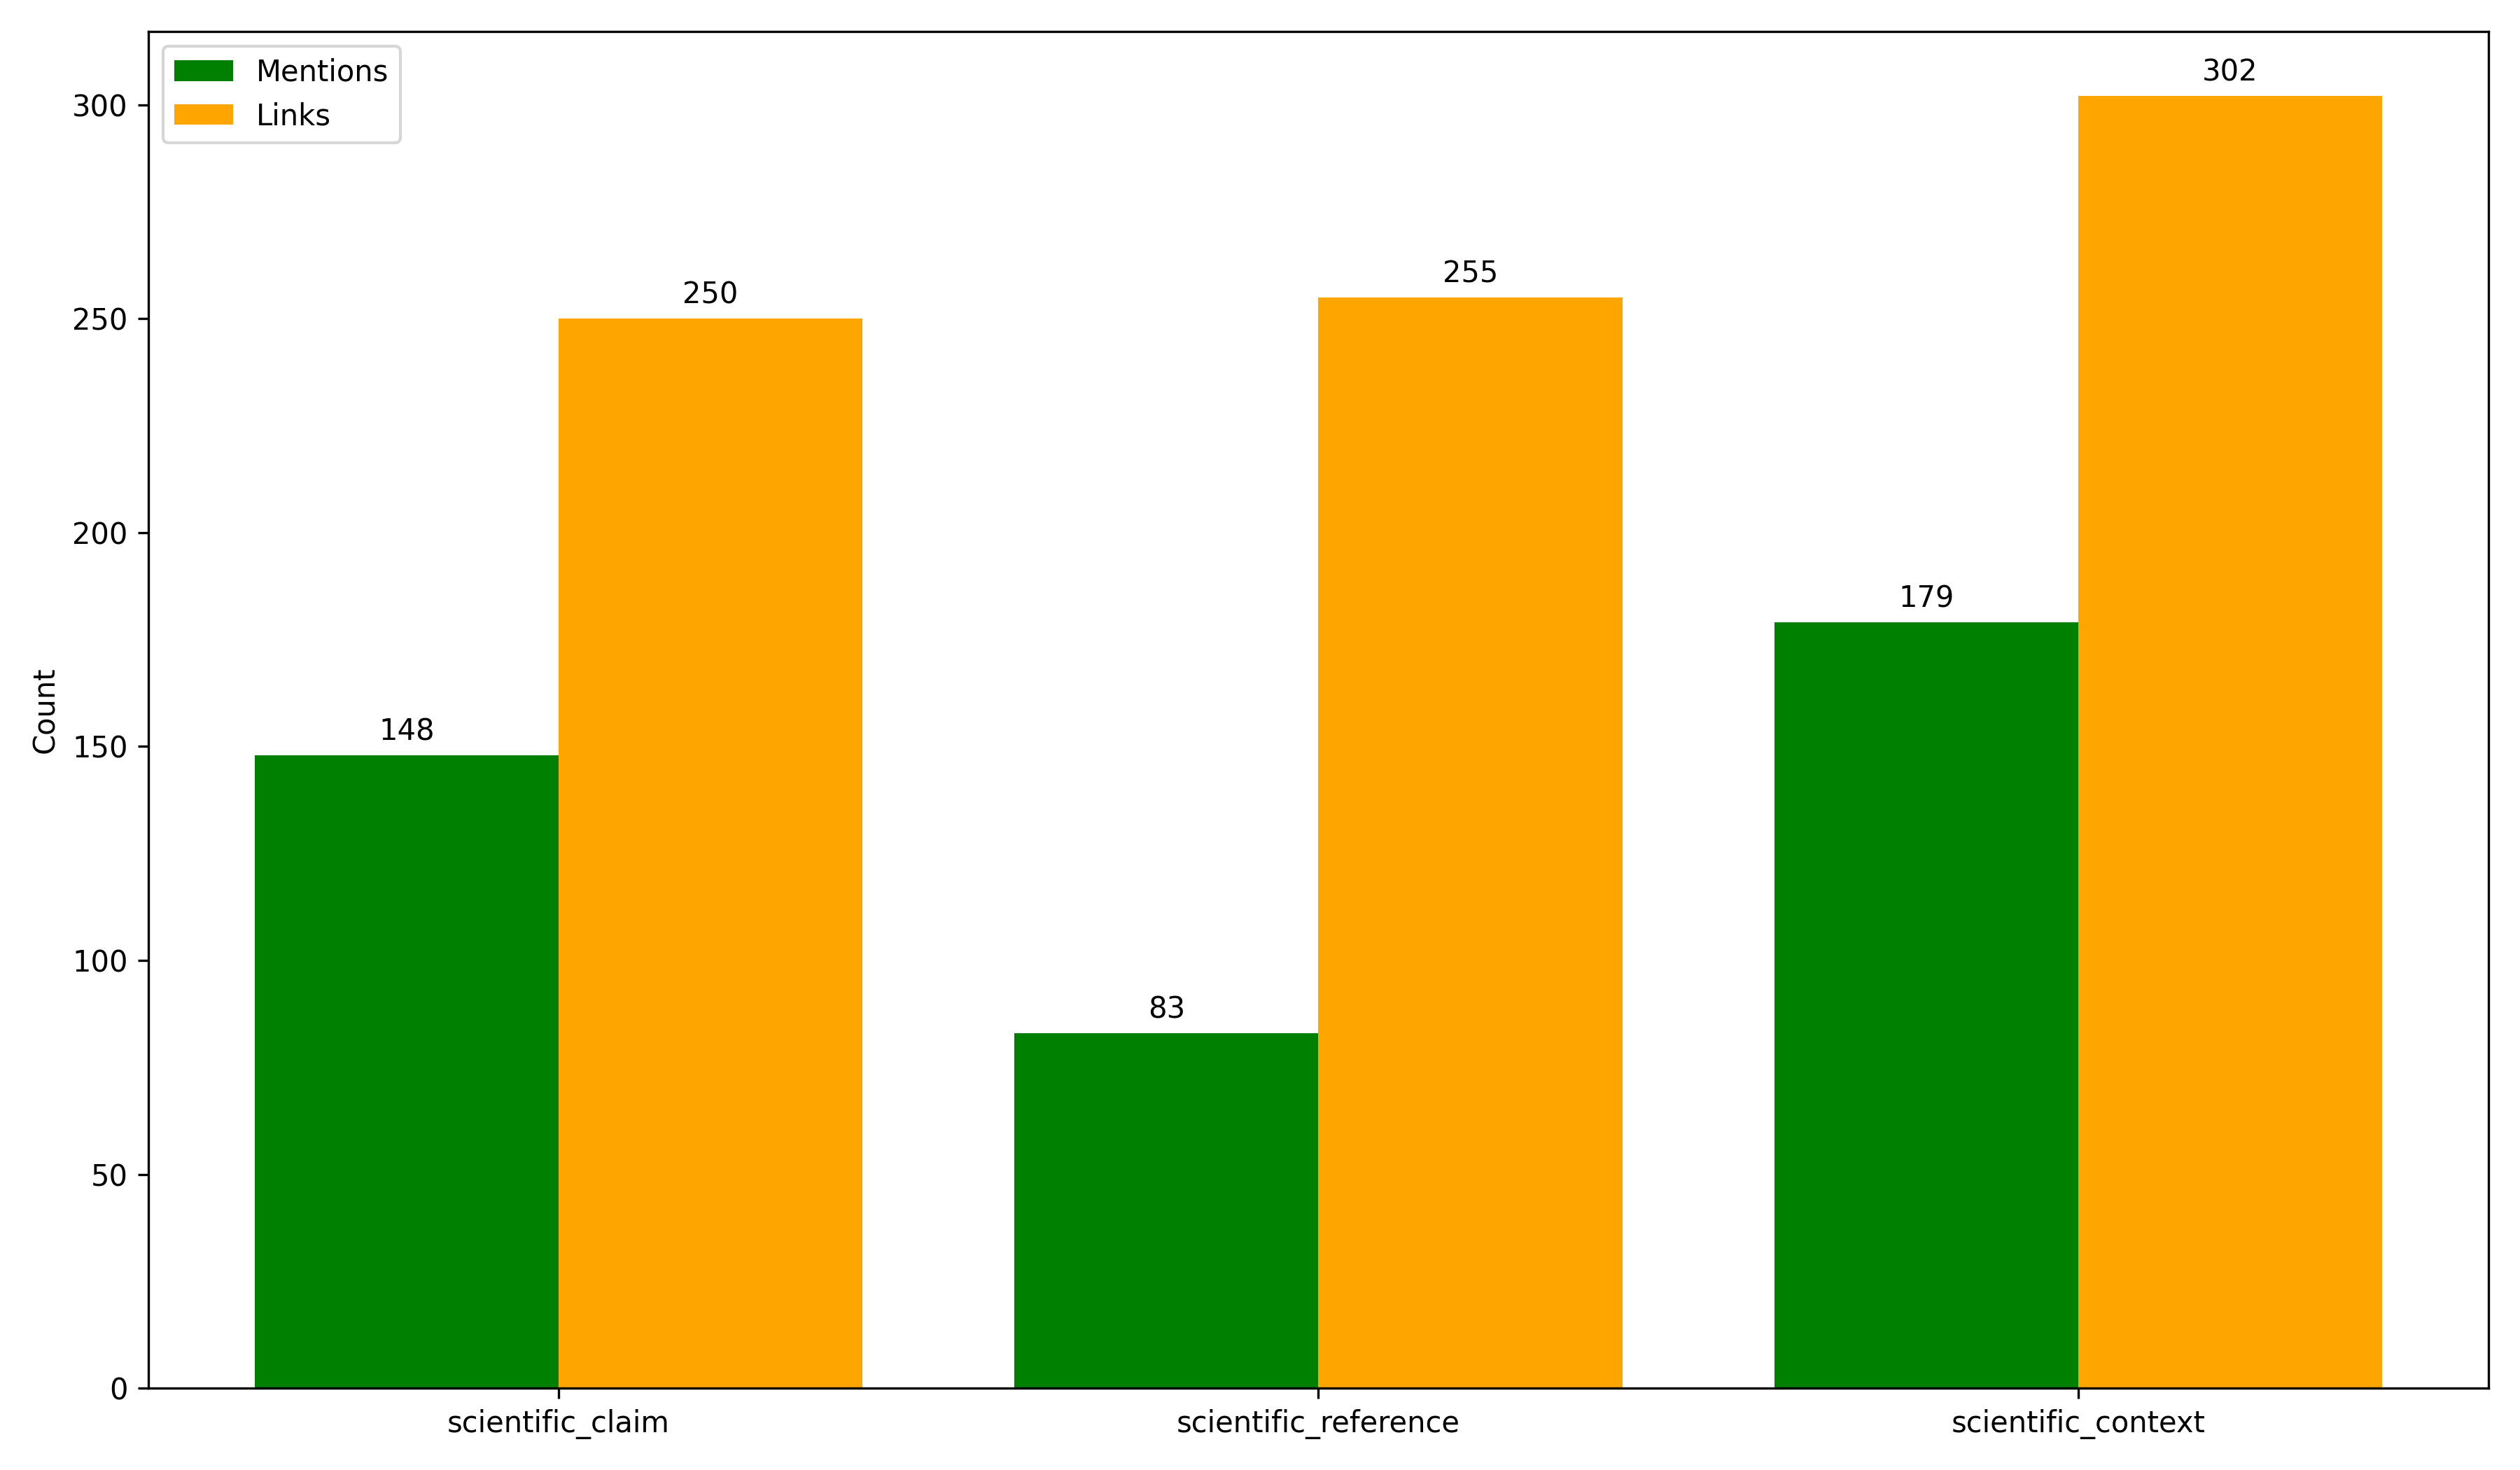
\includegraphics[width=1\textwidth]{images/hashtag_links_mentions_count_outliers}
    \caption{Nombre de hashtags par tweet selon le type de tweet scientifique.}
    \label{fig:hashtag_count}
\end{figure}

Après avoir réalisé des tests d'indépendance de student sur chaque variable, les \textit{p-values} ne descendent pas en dessous de 0.18 donc on ne remarque pas de différence significative entre les tweets scientifiques et non scientifiques.
On peut ainsi conclure que ces variables ne sont pas pertinentes pour la classification des tweets scientifiques, on les retirera de notre dataset.
Malgrès tout, les \texttt{\#} permettent une meilleur accuracy overall, on l'a donc gardé.

    \newpage
    \section{Résultats}\label{sec:results}
    \subsection{Pré-traitement}\label{subsec:pre-traitement}
On regarde le nombre de \texttt{\#}, \texttt{@} et lien par tweet selon le type de tweet scientifique (\autoref{fig:hashtag_count}).

\begin{figure}[H]
    \centering
    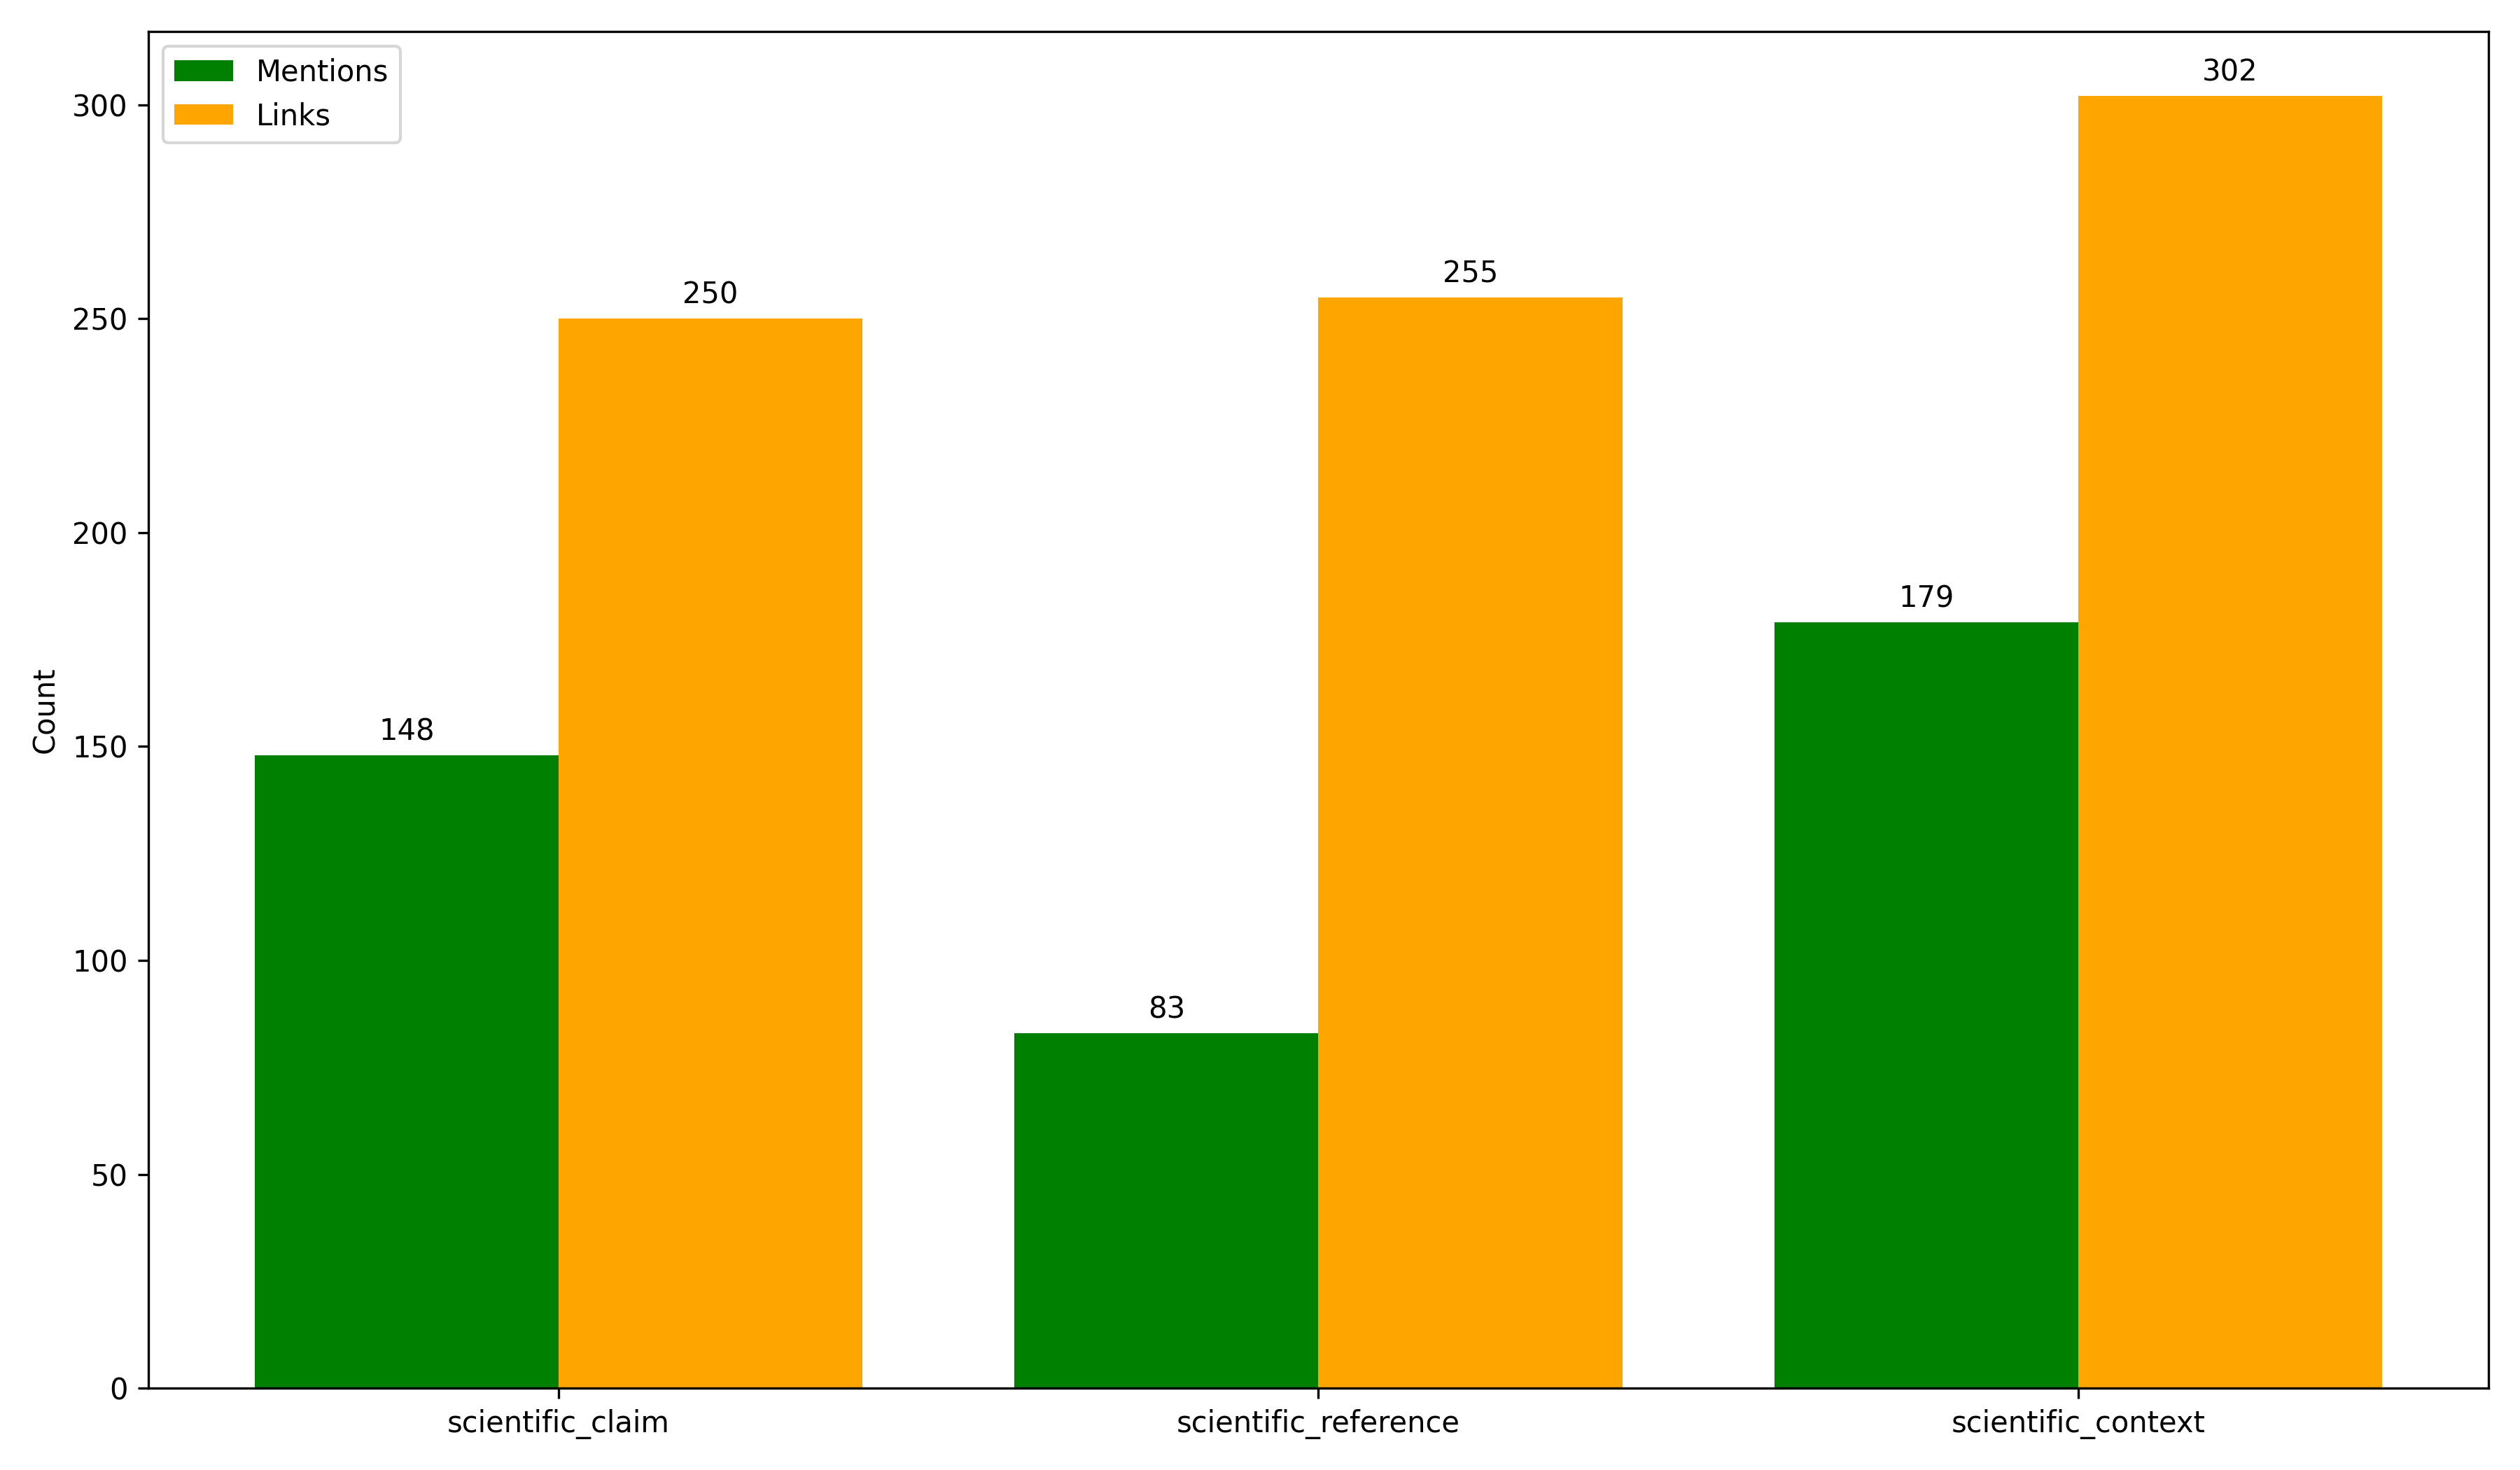
\includegraphics[width=1\textwidth]{images/hashtag_links_mentions_count_outliers}
    \caption{Nombre de hashtags par tweet selon le type de tweet scientifique.}
    \label{fig:hashtag_count}
\end{figure}

Après avoir réalisé des tests d'indépendance de student sur chaque variable, les \textit{p-values} ne descendent pas en dessous de 0.18 donc on ne remarque pas de différence significative entre les tweets scientifiques et non scientifiques.
On peut ainsi conclure que ces variables ne sont pas pertinentes pour la classification des tweets scientifiques, on les retirera de notre dataset.
Malgrès tout, les \texttt{\#} permettent une meilleur accuracy overall, on l'a donc gardé.

\subsection{Modélisation}\label{subsec:modelisation}
Dans cette section, nous comparons les performances des modèles sur trois tâches de classification hiérarchiques successives.
Par la suite, nous présentons les résultats de classification obtenus pour chaque tâche ainsi qu’une comparaison des performances des approches utilisées.

\noindent Pour chacunes des étapes, nous allons comparer différents modèles entre eux pour sélectionner le meilleur modèle.
Par meilleur modèle, on entend la meilleure précision et le plus petit écart-type.
Chaque modèle est testé par cross-validation sur 10 itérations.

\subsection{Modèle 1: Scientifique versus Non Scientifique}\label{subsec:modele-1:-sci-vs-non-sci}
Dans cette tâche, nous avons comparé plusieurs modèles de classification afin de distinguer les tweets scientifiques des non-scientifiques.
L’objectif était d’évaluer les performances de différentes approches d’apprentissage supervisé appliquées à un problème de classification binaire.

\subsubsection{Préparation des données}
Nous avons supprimé les mentions (@), les caractères spéciaux et converti l’ensemble des textes en minuscules, pour standardiser l’entrée pour éviter que des variations superficielles n’influencent la classification.
Une liste de stopwords a été utilisée, combinant celle de NLTK et des termes propres à Twitter ("http", "https", "rt", "co", "amp", "via") qui sont fréquents mais peu informatifs pour déterminer la nature scientifique du contenu.
Pour la vectorisation, nous avons utilisé la méthode TF-IDF avec des n-grammes de taille 1 à 2, un choix raisonnable pour capturer à la fois des mots individuels et des associations fréquentes, tout en limitant la complexité.

Étant donné le fort déséquilibre des classes (la classe SCI représentant moins de 10 \%), la technique SMOTE a été utilisée pour équilibrer la distribution entre classes SCI et NON-SCI.

\subsubsection{Analyse comparative des performances des différents modèles}
Plusieurs modèles de classification ont été testés (\autoref{tab:model_comparison_sci_nsci}).
Chacun a été optimisé à l’aide d’une recherche par grille (GridSearchCV) et évalué à l’aide d’une validation croisée à 10 plis (KFold), afin d’identifier les meilleures combinaisons d’hyperparamètres.

\begin{table}[H]
    \centering
    \caption{Performances des modèles - Tâche 1}
    \begin{tabular}{lcccc}
        \toprule
        Modèle & Accuracy (\autoref{fig:model_comparison_sci_nsci}) & Précision (\autoref{fig:confusion_1.json-logistic-regression_sci_confusion_matrix}) & Rappel (\autoref{fig:confusion_1.json-logistic-regression_sci_confusion_matrix}) & F1-score \\
        \midrule
        Logistic Regression & 0.9327 & 0.93 & 0.93 & 0.93 \\
        Naive Bayes & 0.9092 & 0.91 & 0.90 & 0.90 \\
        k-NN & 0.8092 & 0.83 & 0.80 & 0.80 \\
        Random Forest & 0.8680 & 0.86 & 0.84 & 0.83 \\
        SVM (linéaire) & 0.9412 & 0.94 & 0.94 & 0.94 \\
        \bottomrule
    \end{tabular}\label{tab:model_comparison_sci_nsci}
\end{table}

\noindent Le modèle SVM semble être le plus performant pour cette tâche, affichant les meilleurs scores en précision, rappel et F1-score, ainsi qu’une accuracy élevée accompagnée mais un plus grand écart-type que la régression logistique \autoref{fig:model_comparison_sci_nsci}.
C'est pour cette raison de stabilité que l'on préfèrera la régression logistique car elle présente une baisse de performance négligeable comparé à la stabilité du modèle.

\begin{figure}[H]
    \centering
    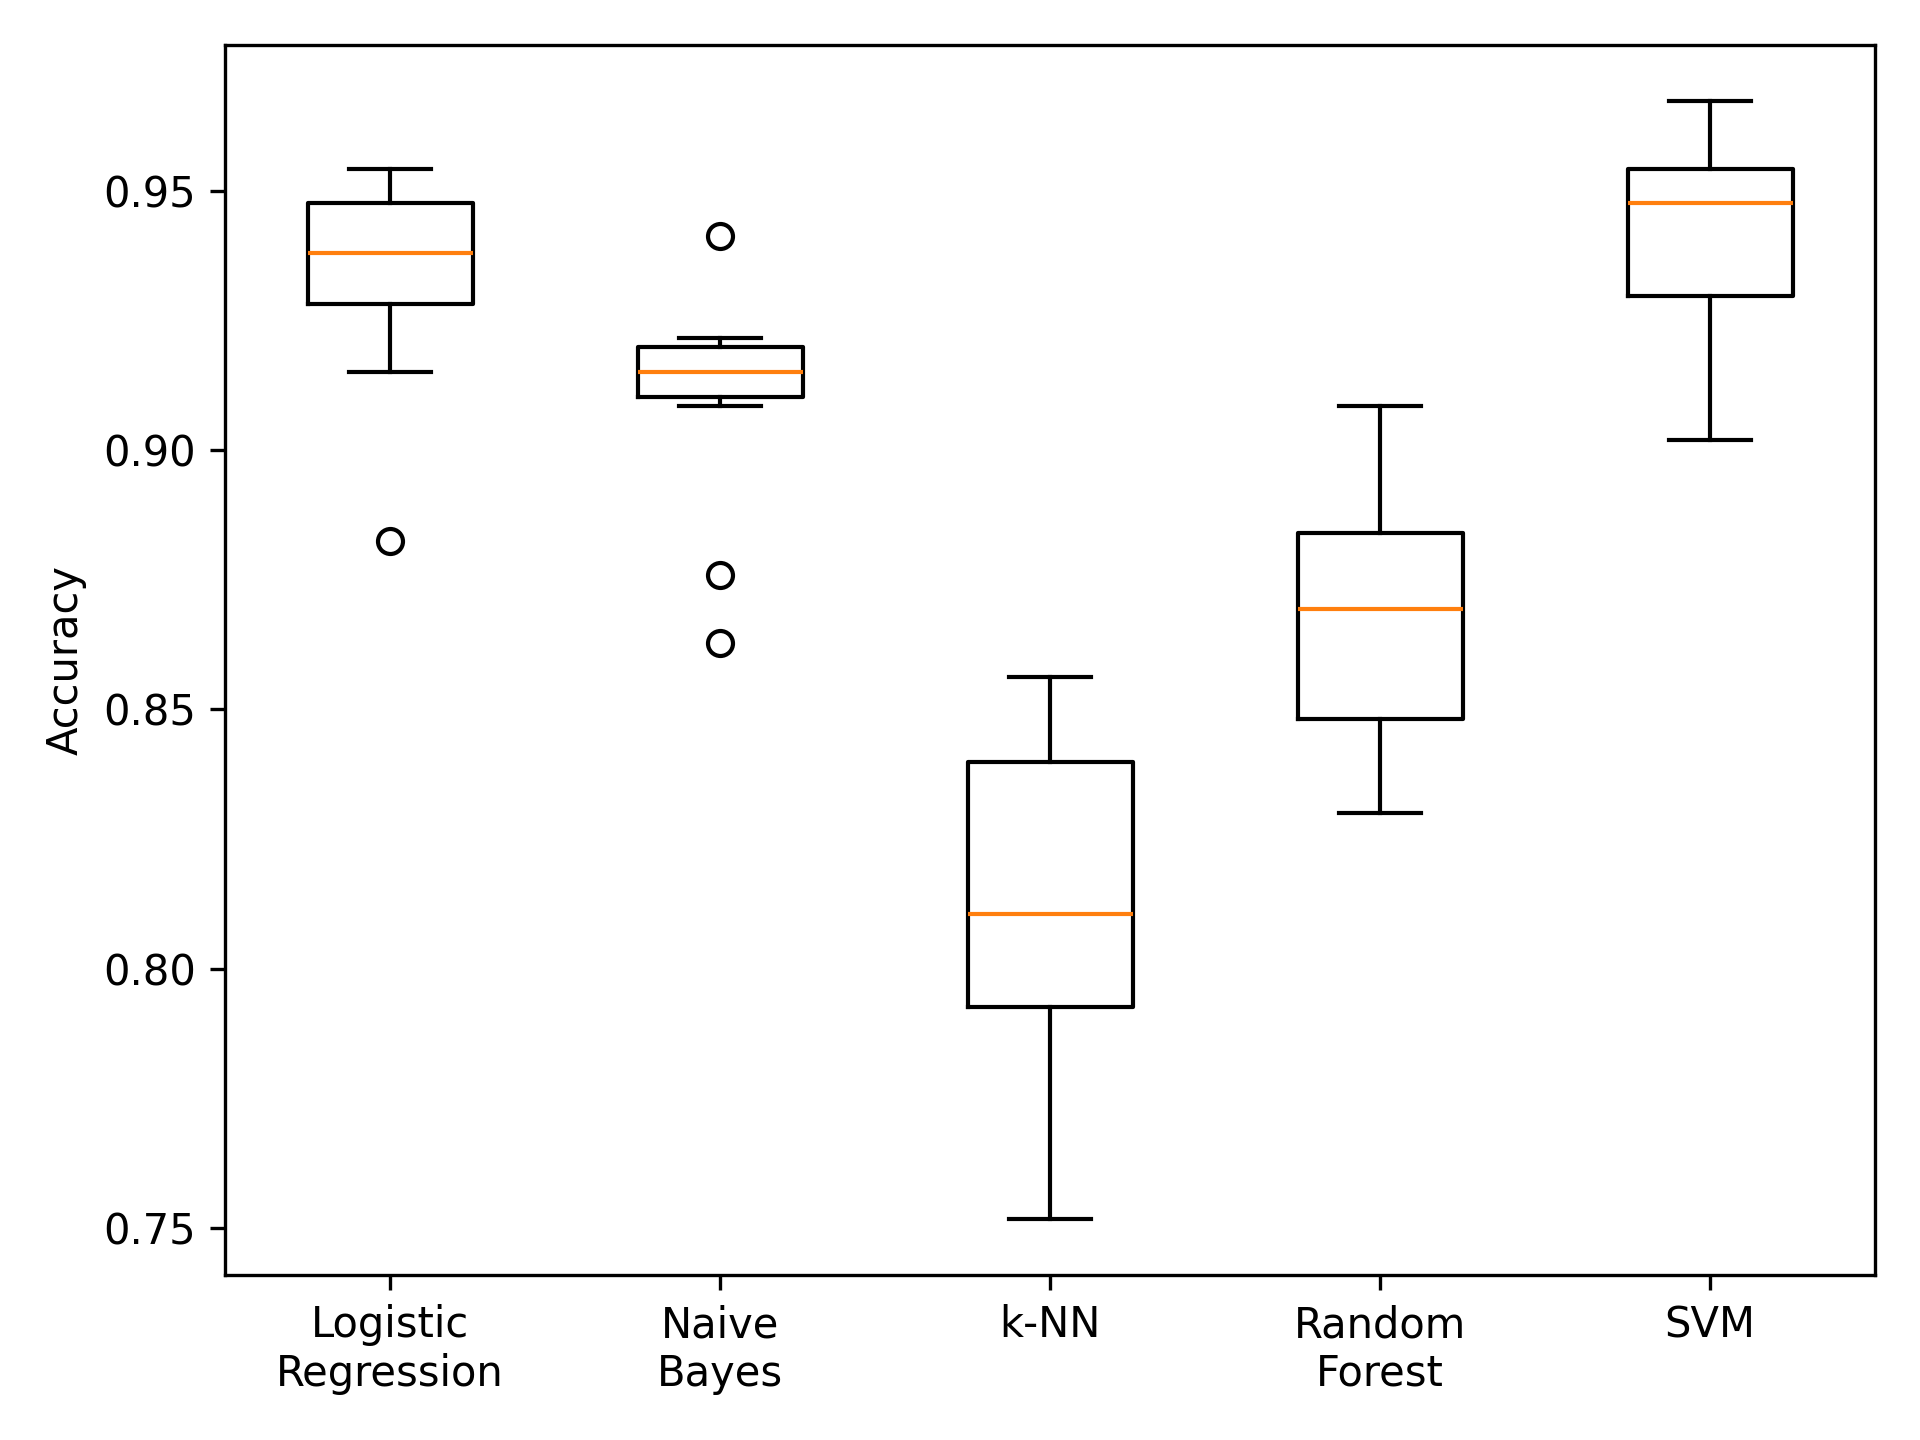
\includegraphics[width=0.75\textwidth]{images/model_comparison_1}
    \caption{Comparaison des modèles pour la classification des tweets scientifiques et non scientifiques.}
    \label{fig:model_comparison_sci_nsci}
\end{figure}

\begin{figure}[H]
    \centering
    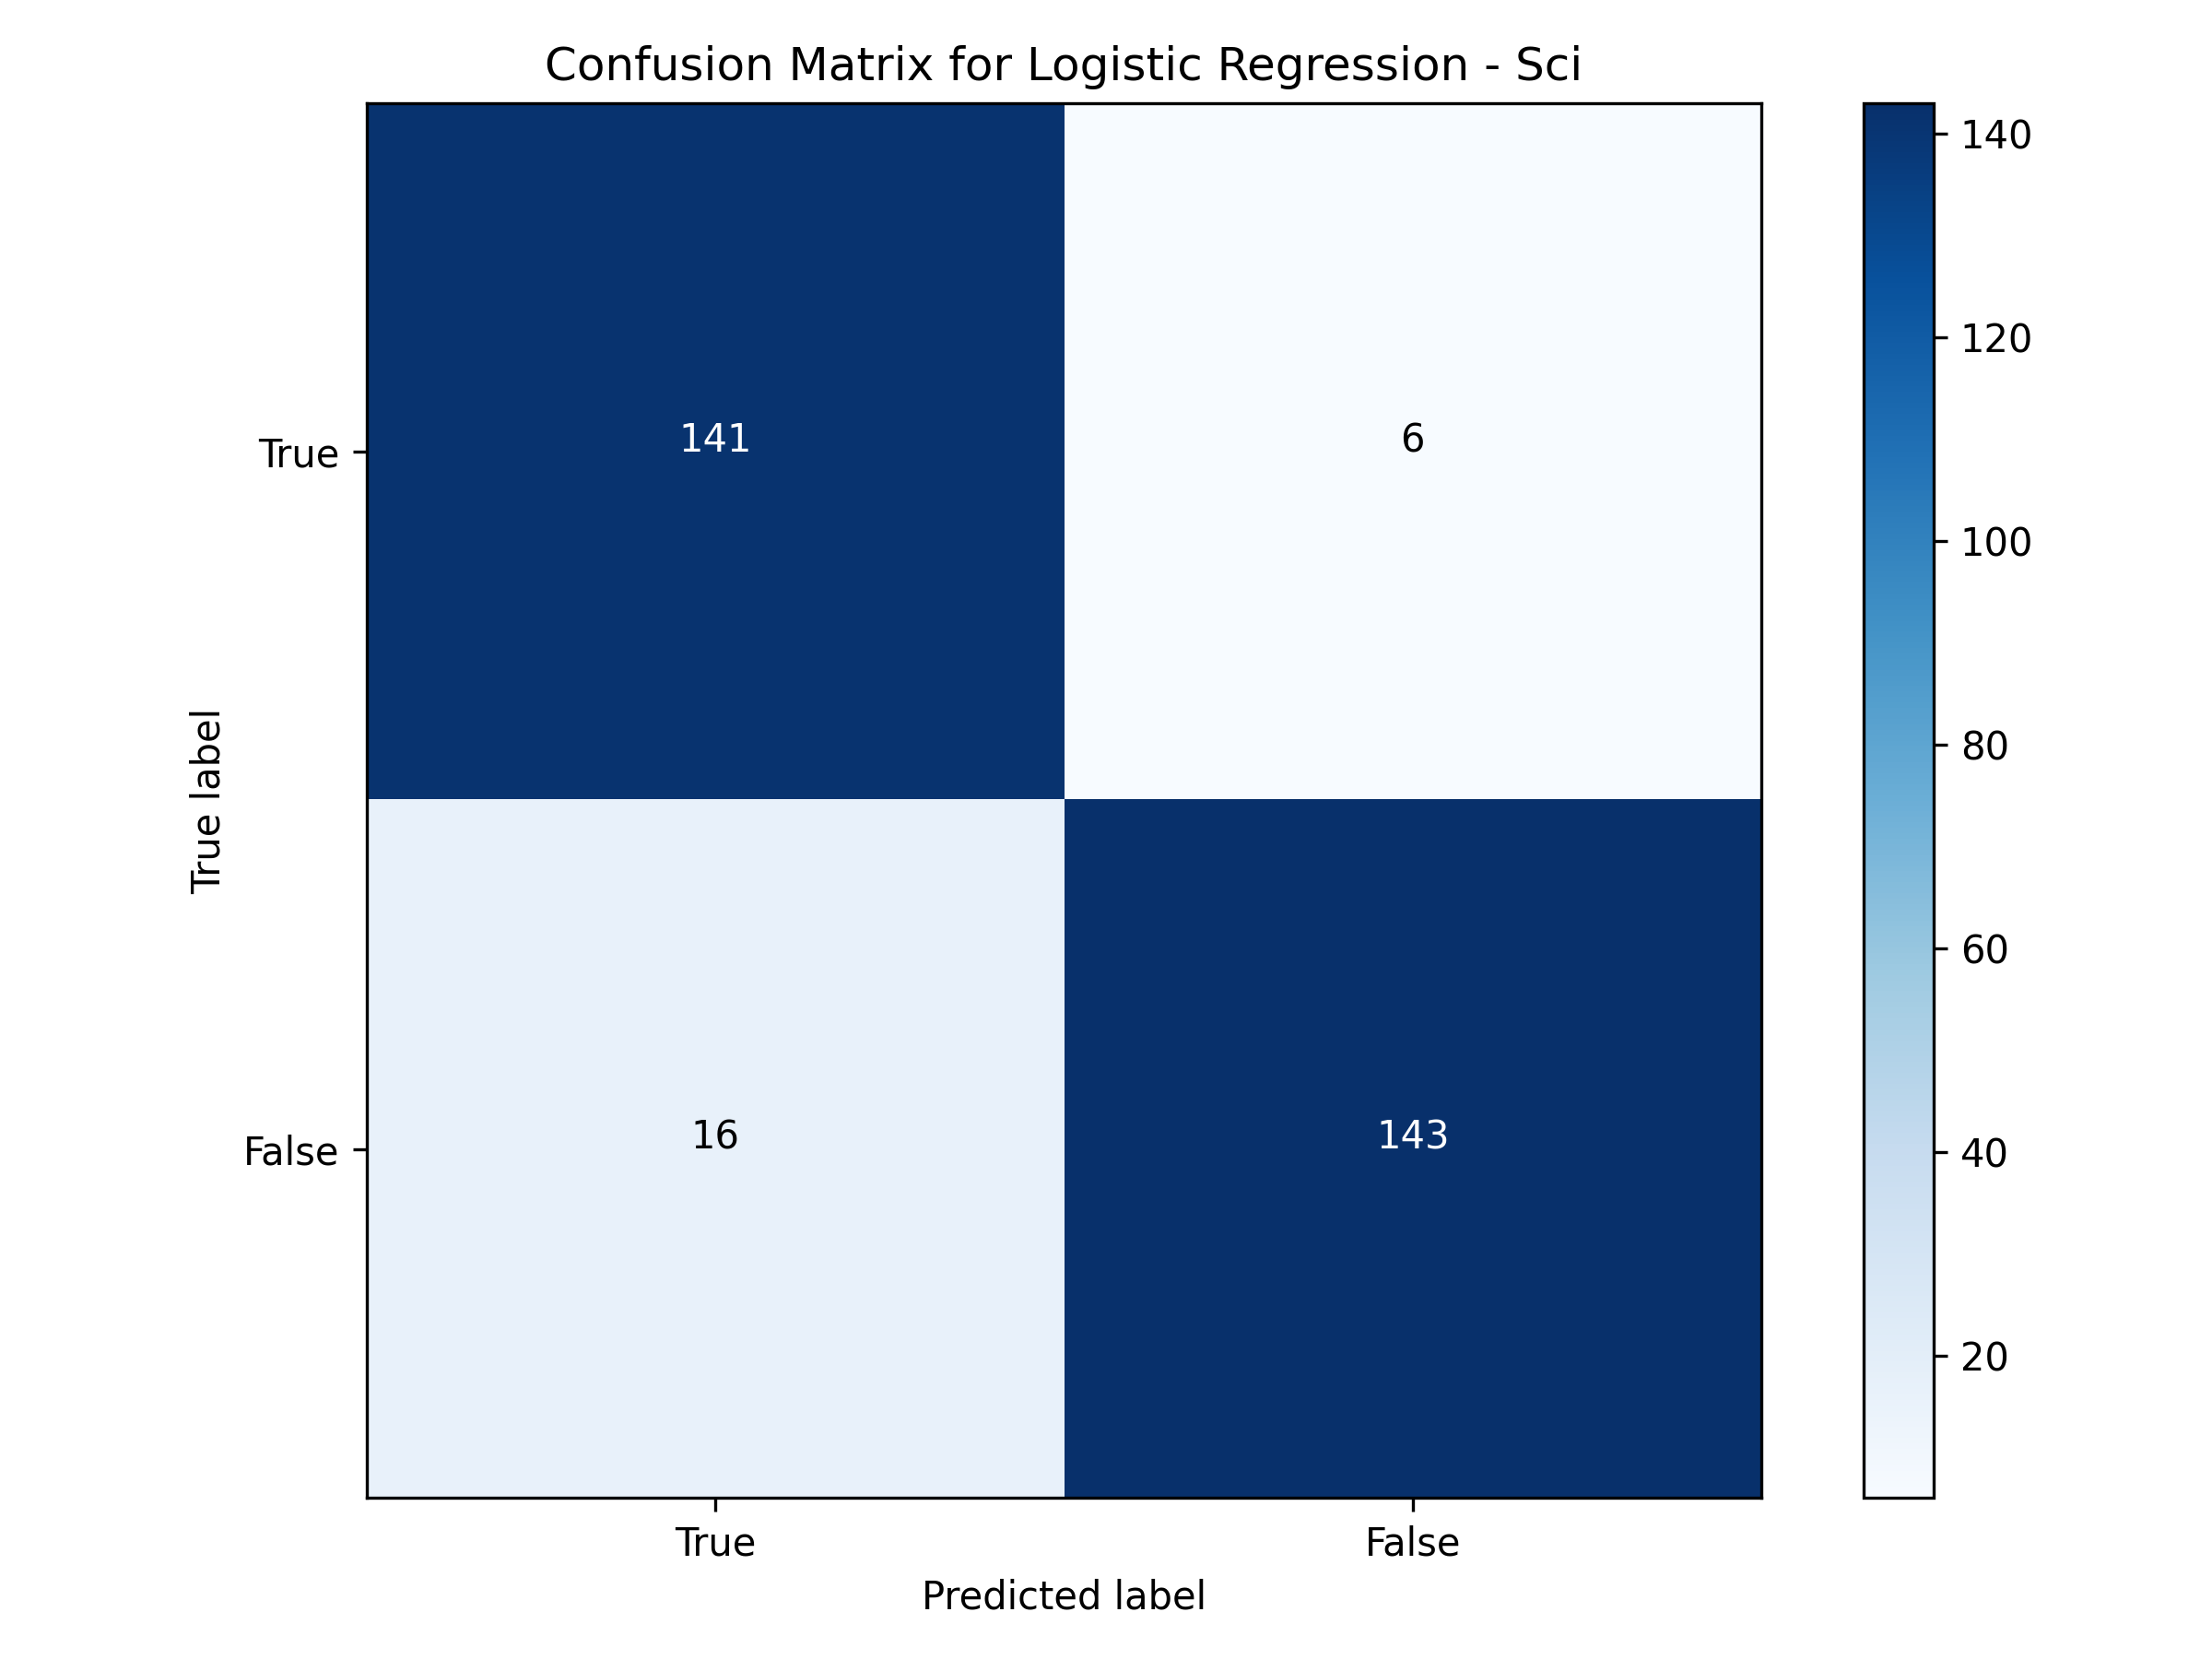
\includegraphics[width=0.49\textwidth]{images/confusion_1.json-Logistic Regression_Sci_confusion_matrix}
    \caption{Matrice de confusion du modèle Logistic Regression pour la classification des tweets scientifiques et non scientifiques.}
    \label{fig:confusion_1.json-logistic-regression_sci_confusion_matrix}
\end{figure}

\subsection{Modèle 2: Affirmation et Référence versus Contexte}\label{subsec:modele-2:-claim-et-ref-vs-contexte}
À présent, nous allons considérer les classes "Affirmation" et "Référence" qui citent une affirmation scientifique d’une part, et la classe "Contexte" qui servent de contexte
D’autre part, toujours afin de réaliser une classification binaire.
Les tweets analysés sont uniquement ceux classés comme scientifiques dans la première tâche.

\subsubsection{Préparation des données}
Le prétraitement textuel a suivi une logique proche de celle adoptée dans la première tâche (minuscules, stop words, lemmatisation), mais sans suppression des mentions et caractères 	spéciaux, afin d’explorer s’ils peuvent porter une valeur contextuelle utile.

La vectorisation a été réalisée à l’aide de TF-IDF, en élargissant la fenêtre aux trigrammes (1 à 3-grammes) afin de mieux capturer les structures linguistiques propres aux énoncés de type affirmation ou citation.

Contrairement à la première tâche, nous n’avons pas appliqué SMOTE Ici, le déséquilibre est partiel dans la distribution des combinaisons de labels (tableau 2,) car la combinaison {1,1} est majoritaire, tandis que la combinaison {0,1} est fortement sous-représentée. La classification est multi-label (un tweet 	peut être à la fois CONTEXT et CLAIM/REF). Nous avons donc  implémenté un rééchantillonnage manuel spécifique au multi-label, en nous basant sur l’identification de toutes les combinaisons de labels possibles et en suréchantillonnant celles qui étaient sous-représentées. 
\begin{figure}[H]
    \centering
    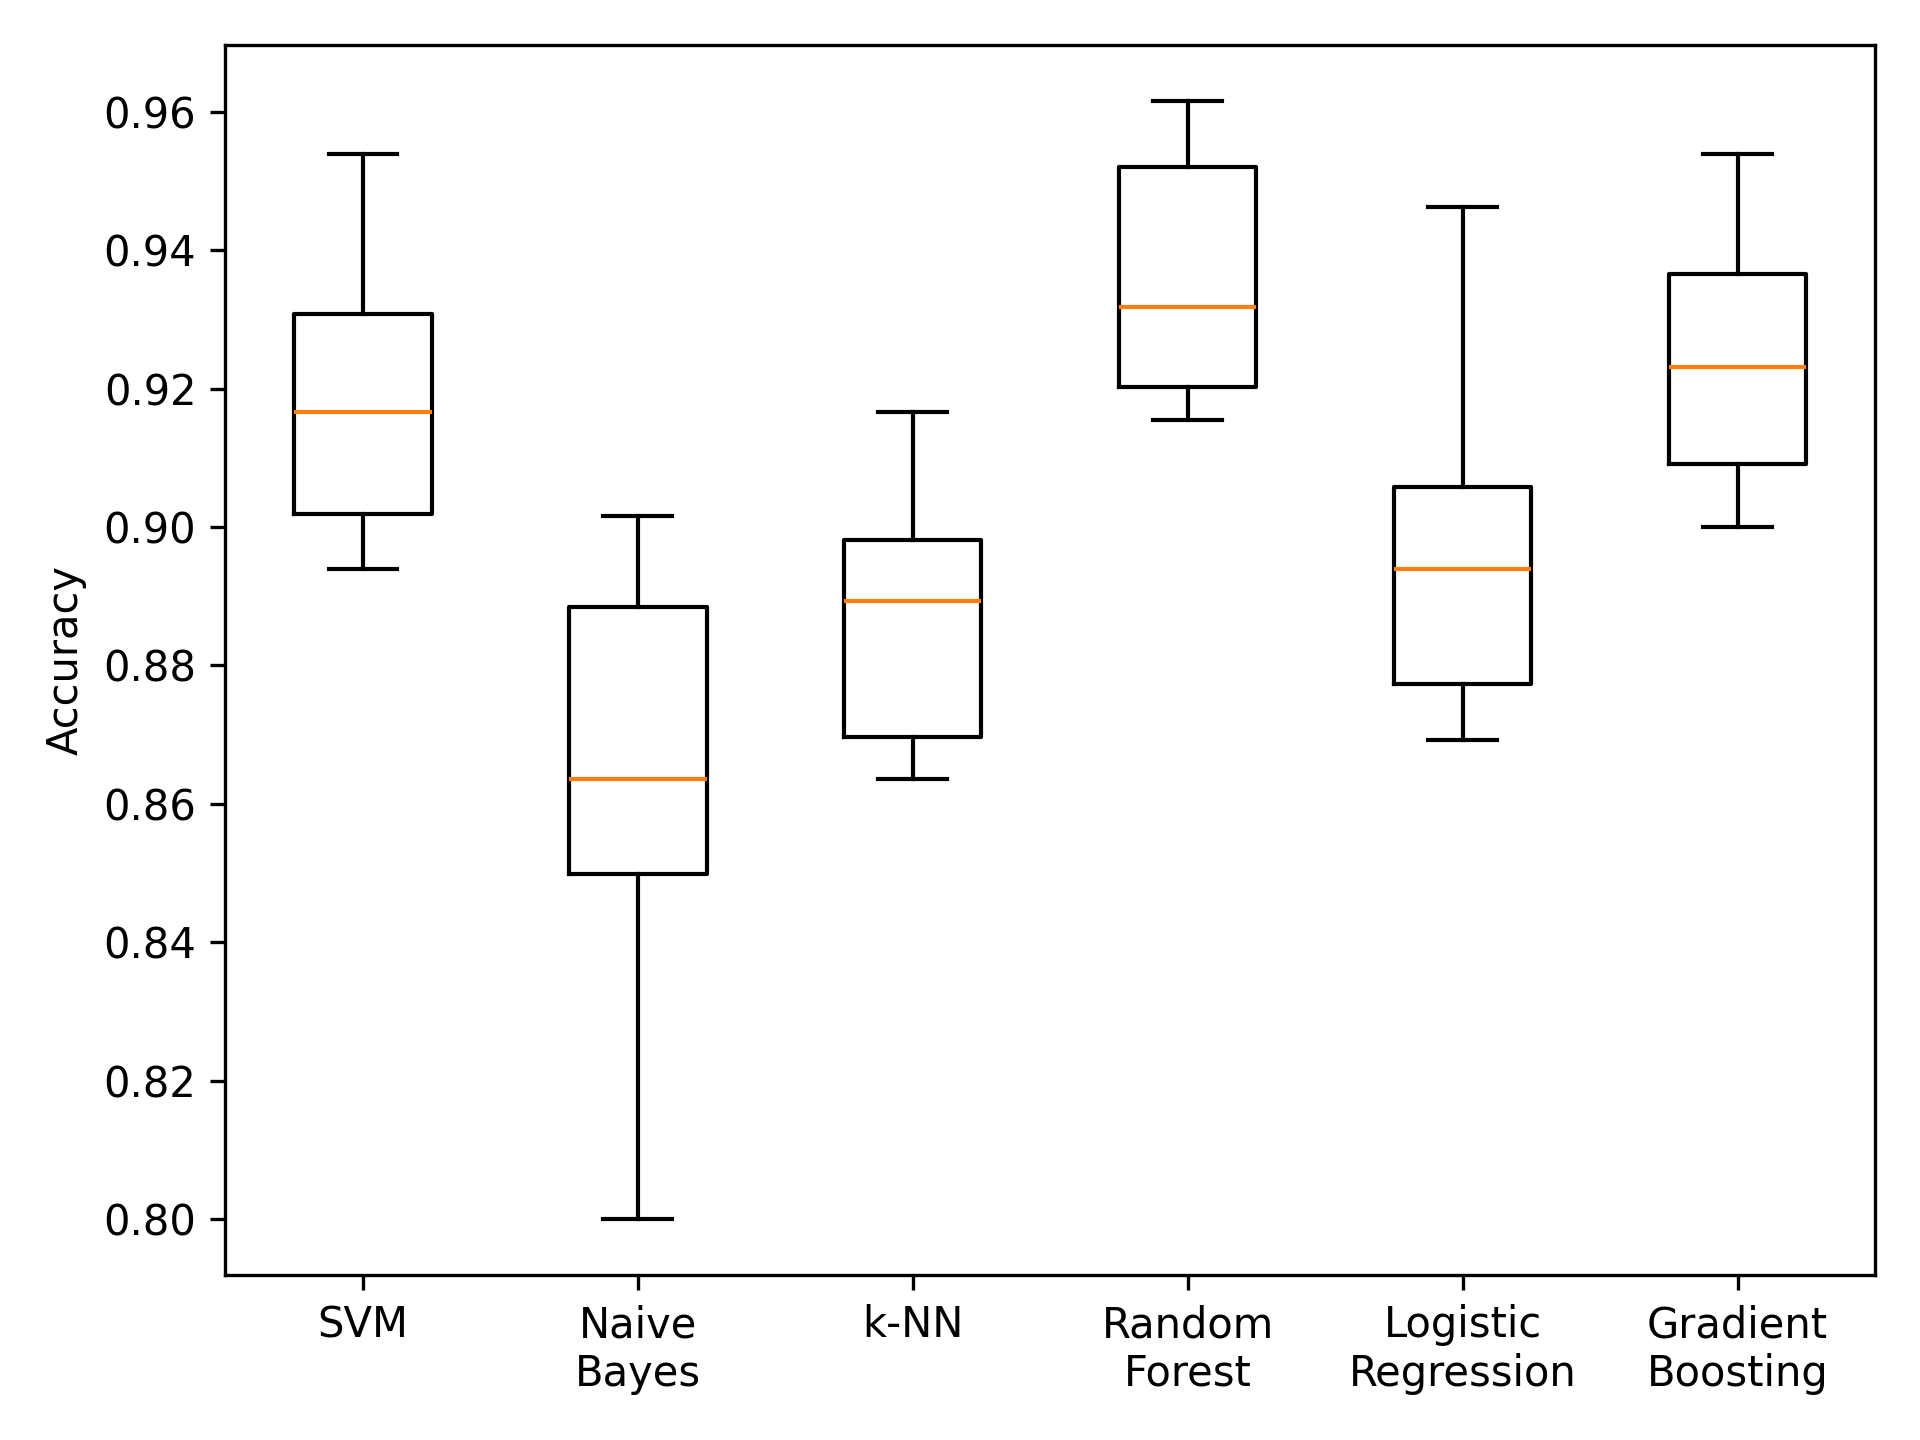
\includegraphics[width=0.75\textwidth]{images/model_comparison_2}
    \caption{Comparaison des modèles pour la classification des tweets claim et ref vs contexte.}
    \label{fig:model_comparison_clmref_context}
\end{figure}

\begin{figure}[h]
    \centering
    \begin{minipage}[b]{0.49\textwidth}
        \centering
        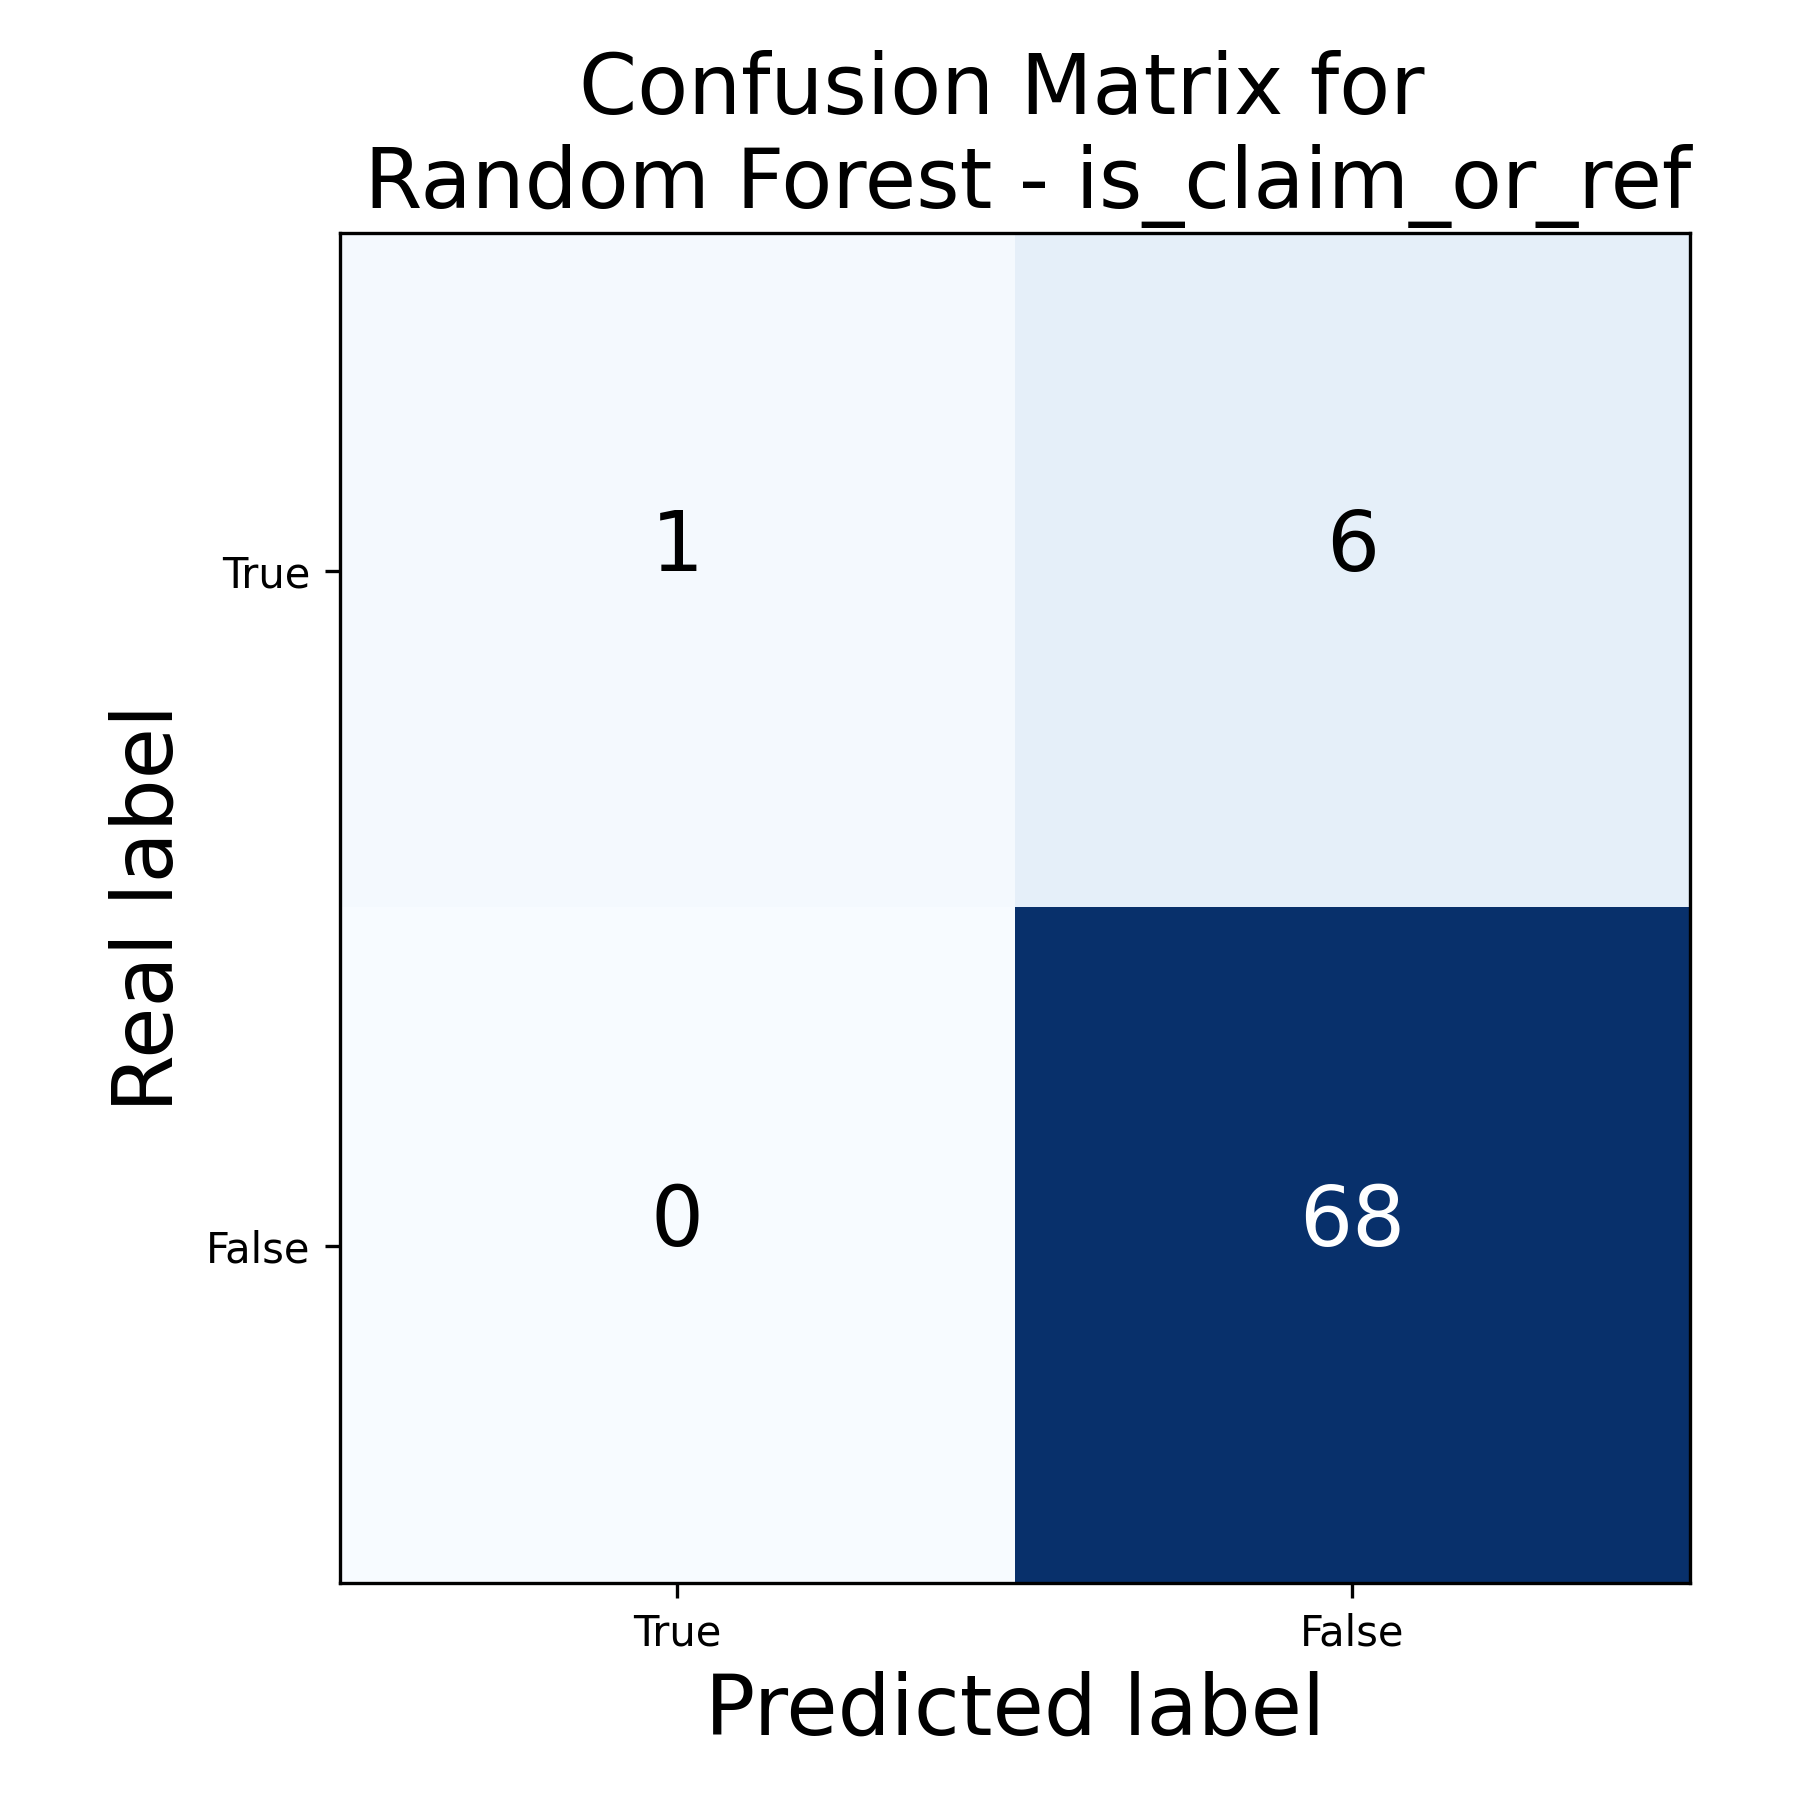
\includegraphics[width=\textwidth]{images/confusion_2.json-Random Forest_is_claim_or_ref_confusion_matrix}
        \label{fig:confusion_2_1}
    \end{minipage}
    \hfill
    \begin{minipage}[b]{0.49\textwidth}
        \centering
        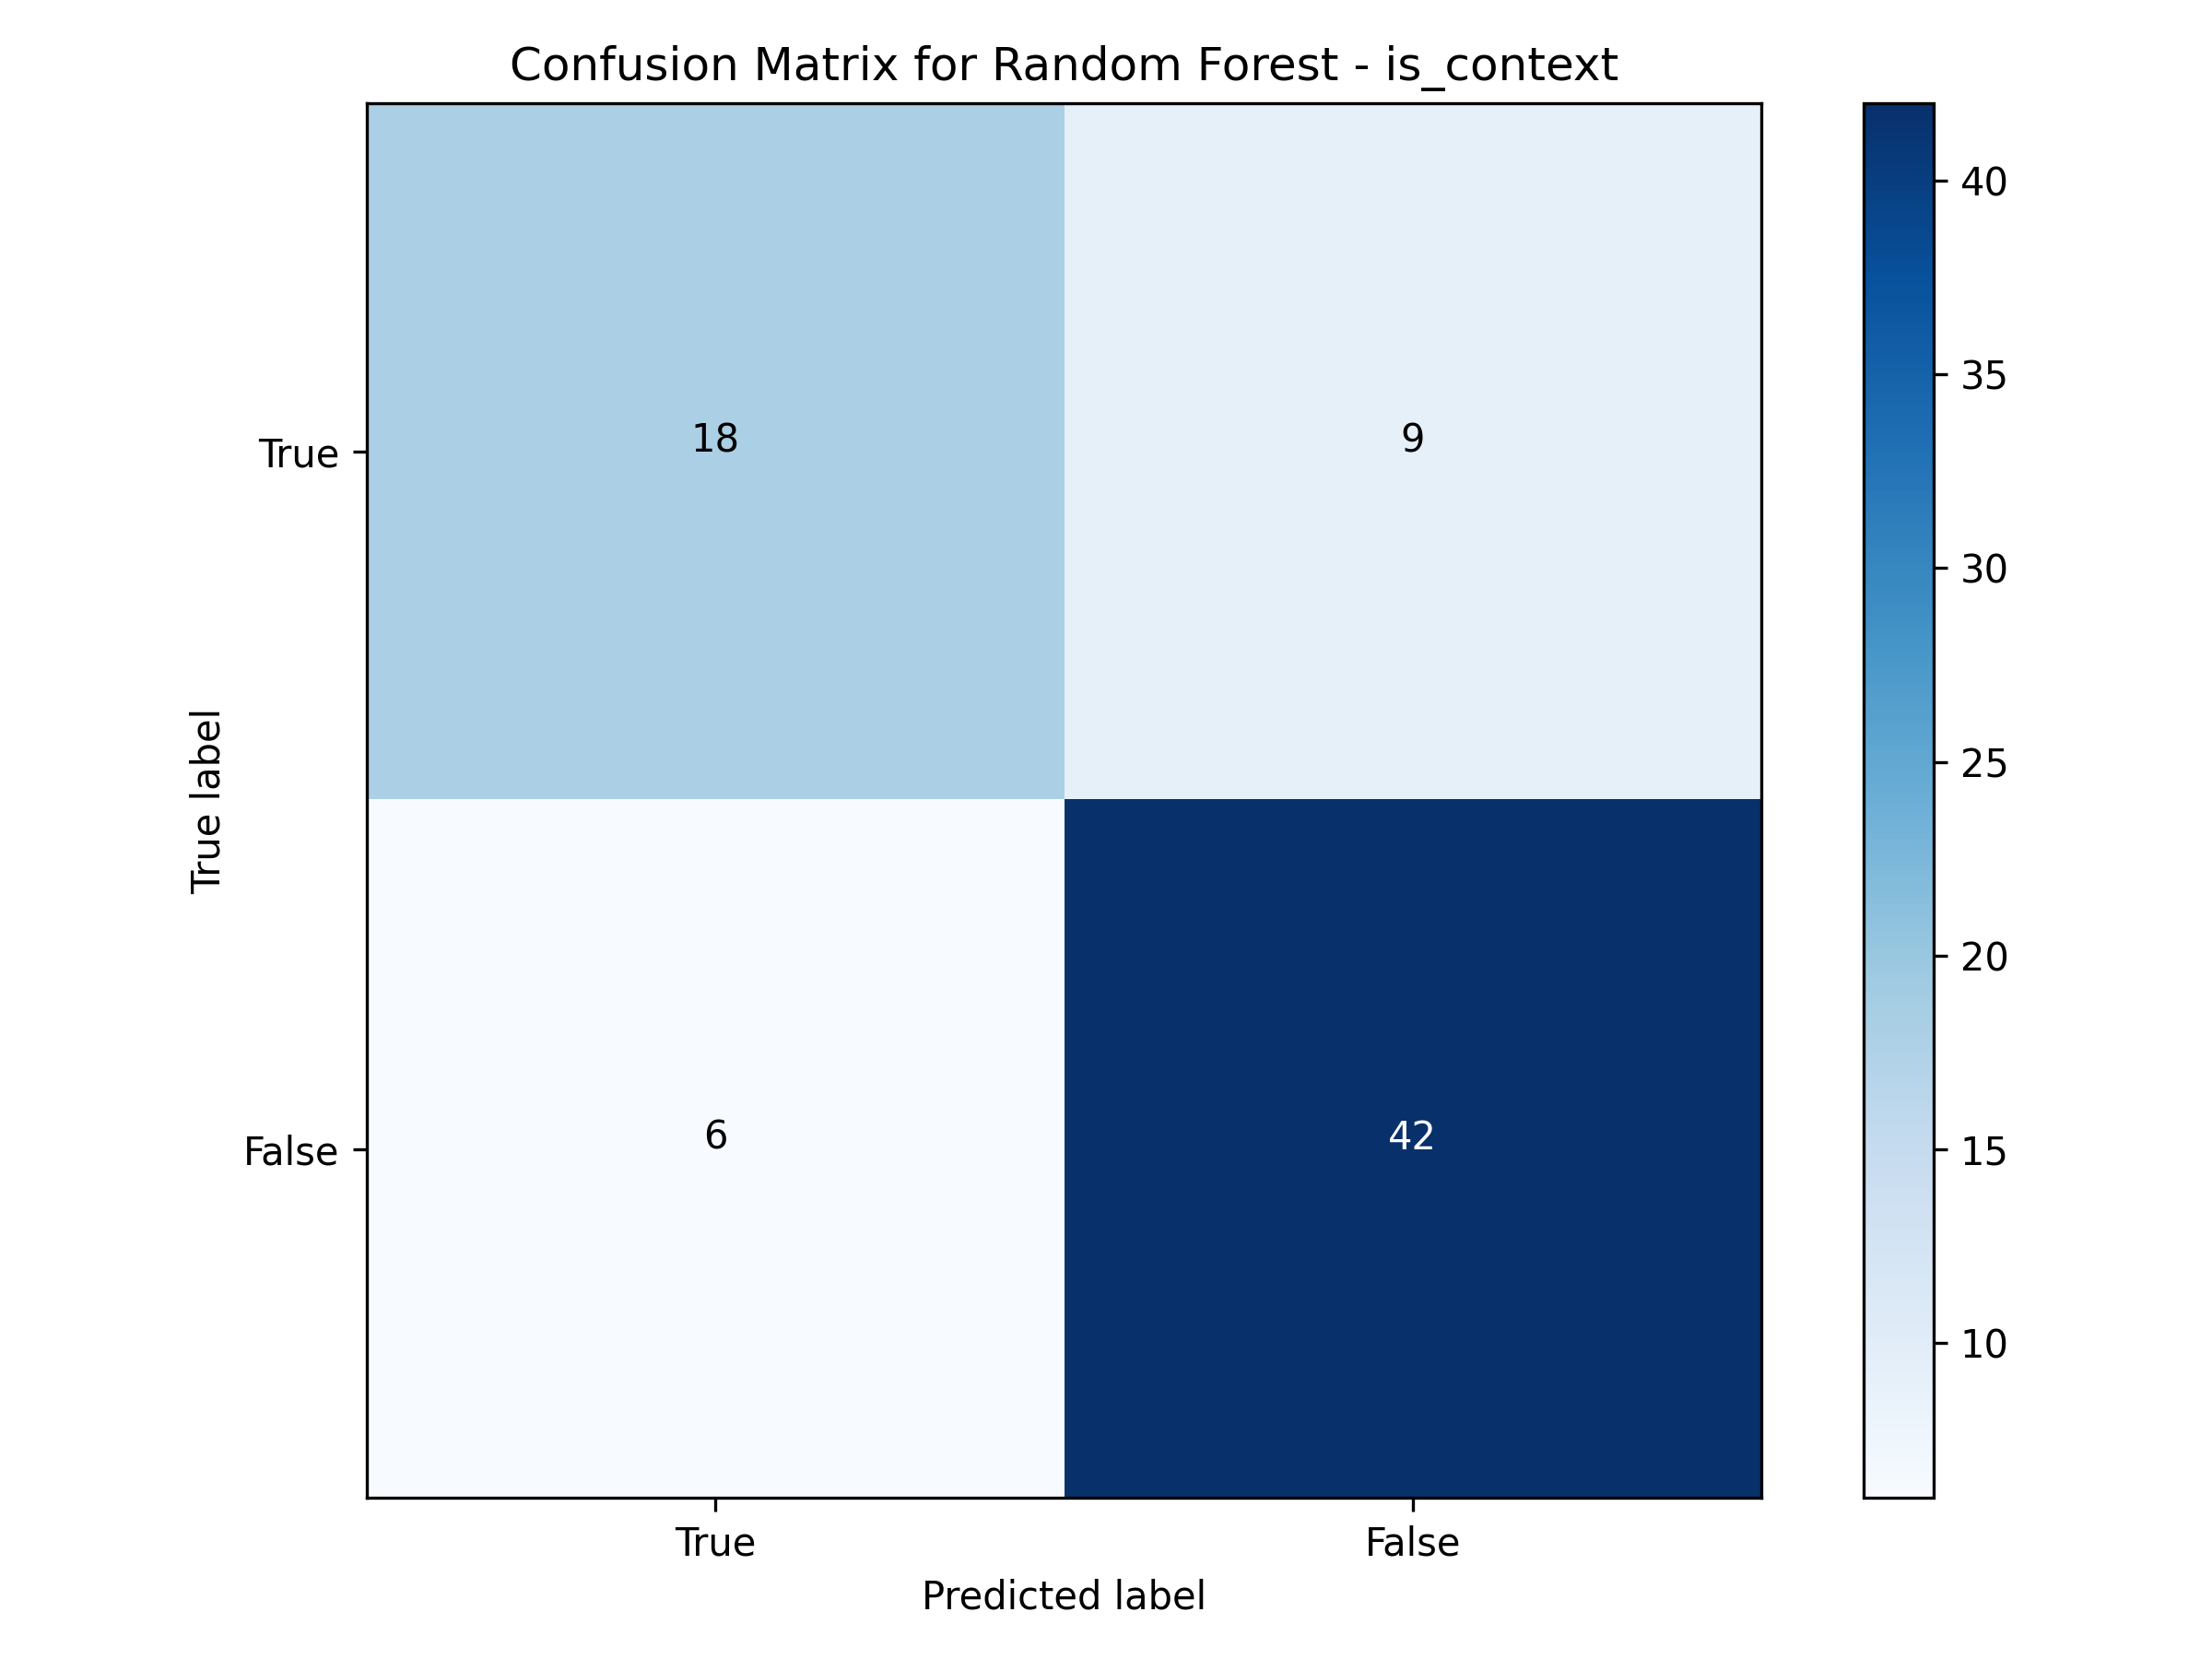
\includegraphics[width=\textwidth]{images/confusion_2.json-Random Forest_is_context_confusion_matrix}
        \label{fig:confusion_2_2}
    \end{minipage}
    \caption{Matrice de confusion du modèle Random Forest pour la classification des tweets claim et ref vs contexte.}
    \label{fig:confusion_2}
\end{figure}

\subsection{Modèle 3: claim vs ref vs contexte}\label{subsec:modele-3:-claim-vs-ref-vs-contexte}
\begin{figure}[H]
    \centering
    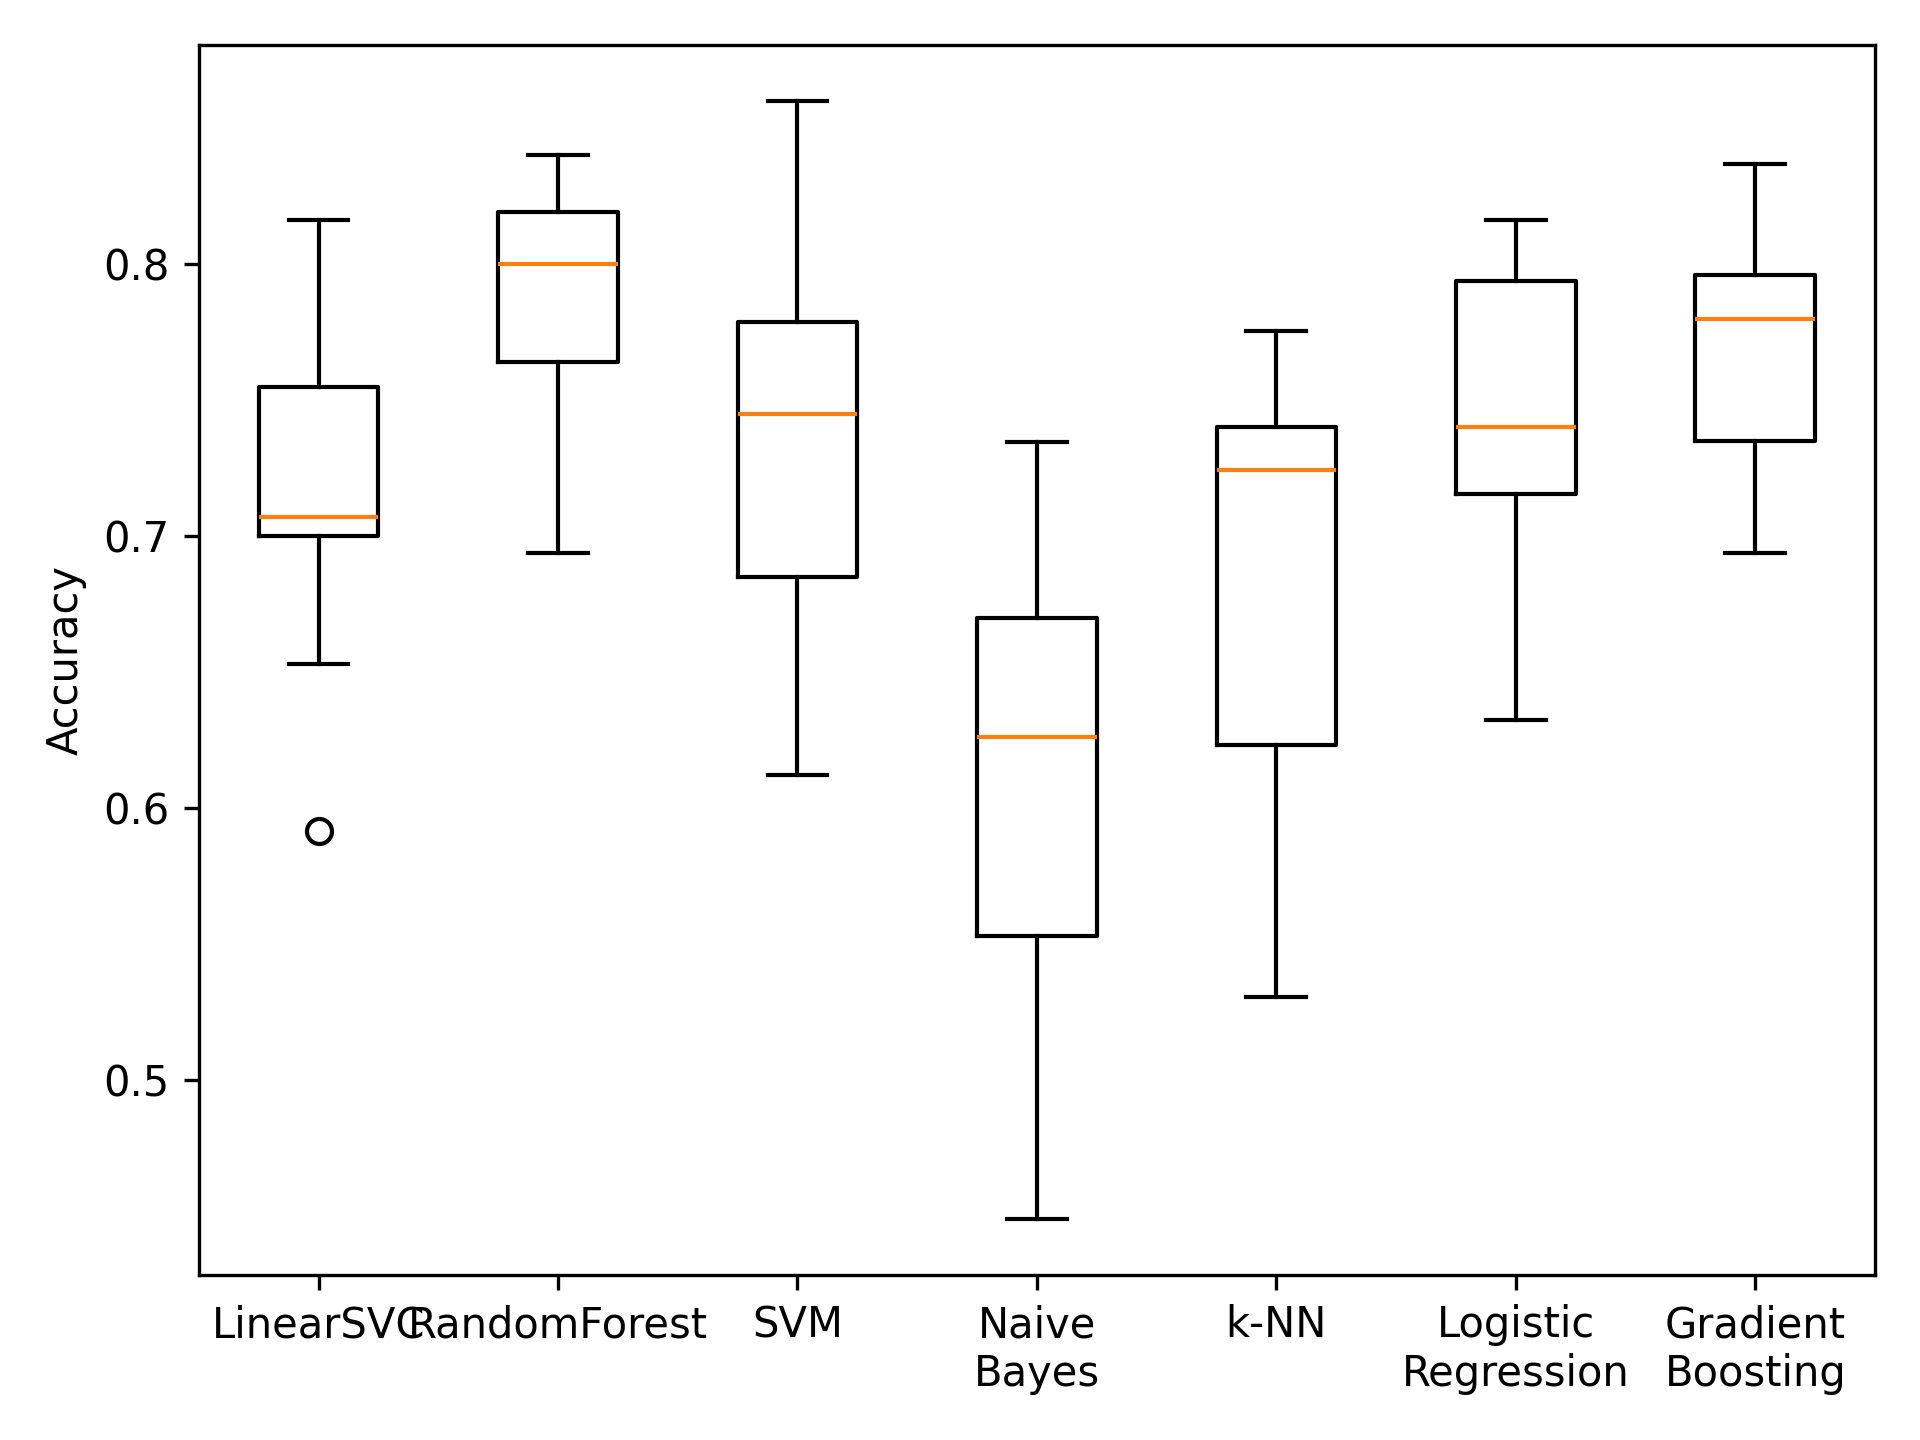
\includegraphics[width=0.75\textwidth]{images/model_comparison_3}
    \caption{Comparaison des modèles pour la classification des tweets claim vs ref vs contexte.}
    \label{fig:model_comparison_clm_ref_context}
\end{figure}

\begin{figure}[h]
    \centering
    \begin{minipage}[b]{0.45\textwidth}
        \centering
        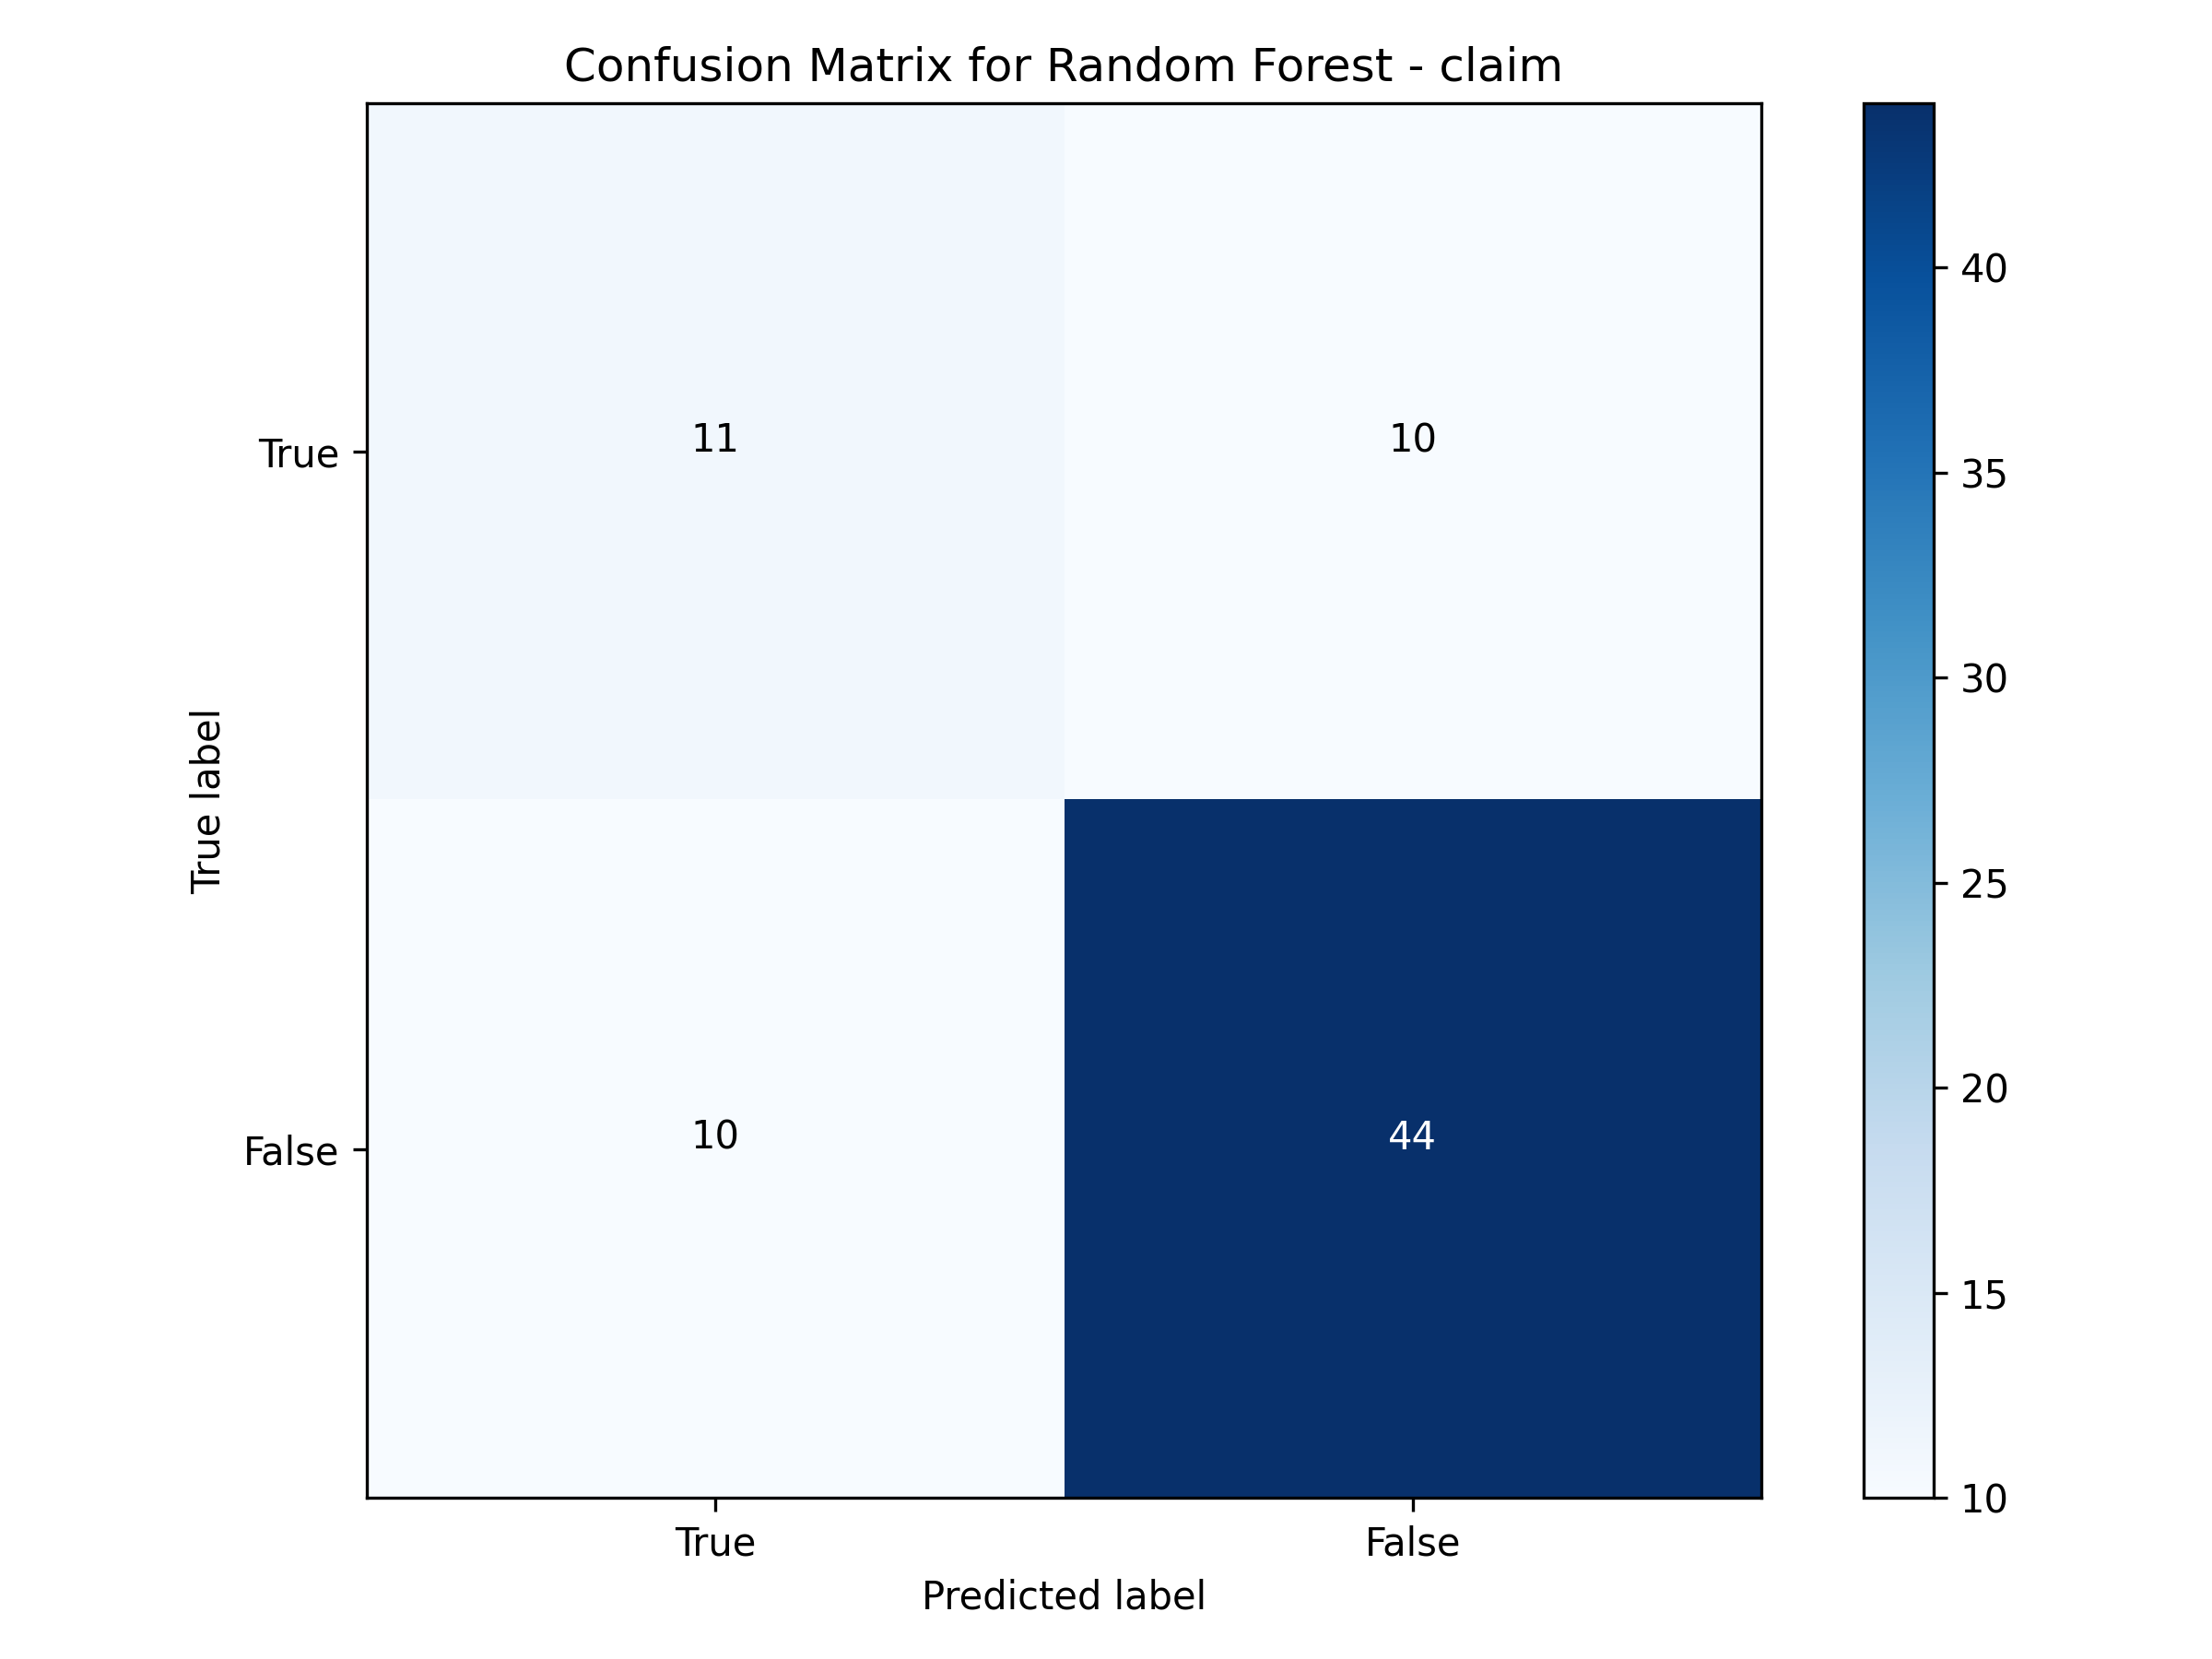
\includegraphics[width=\textwidth]{images/confusion_3.json-Random Forest_claim_confusion_matrix}
        \label{fig:confusion_3_1}
    \end{minipage}
    \hspace{1em}
    \begin{minipage}[b]{0.45\textwidth}
        \centering
        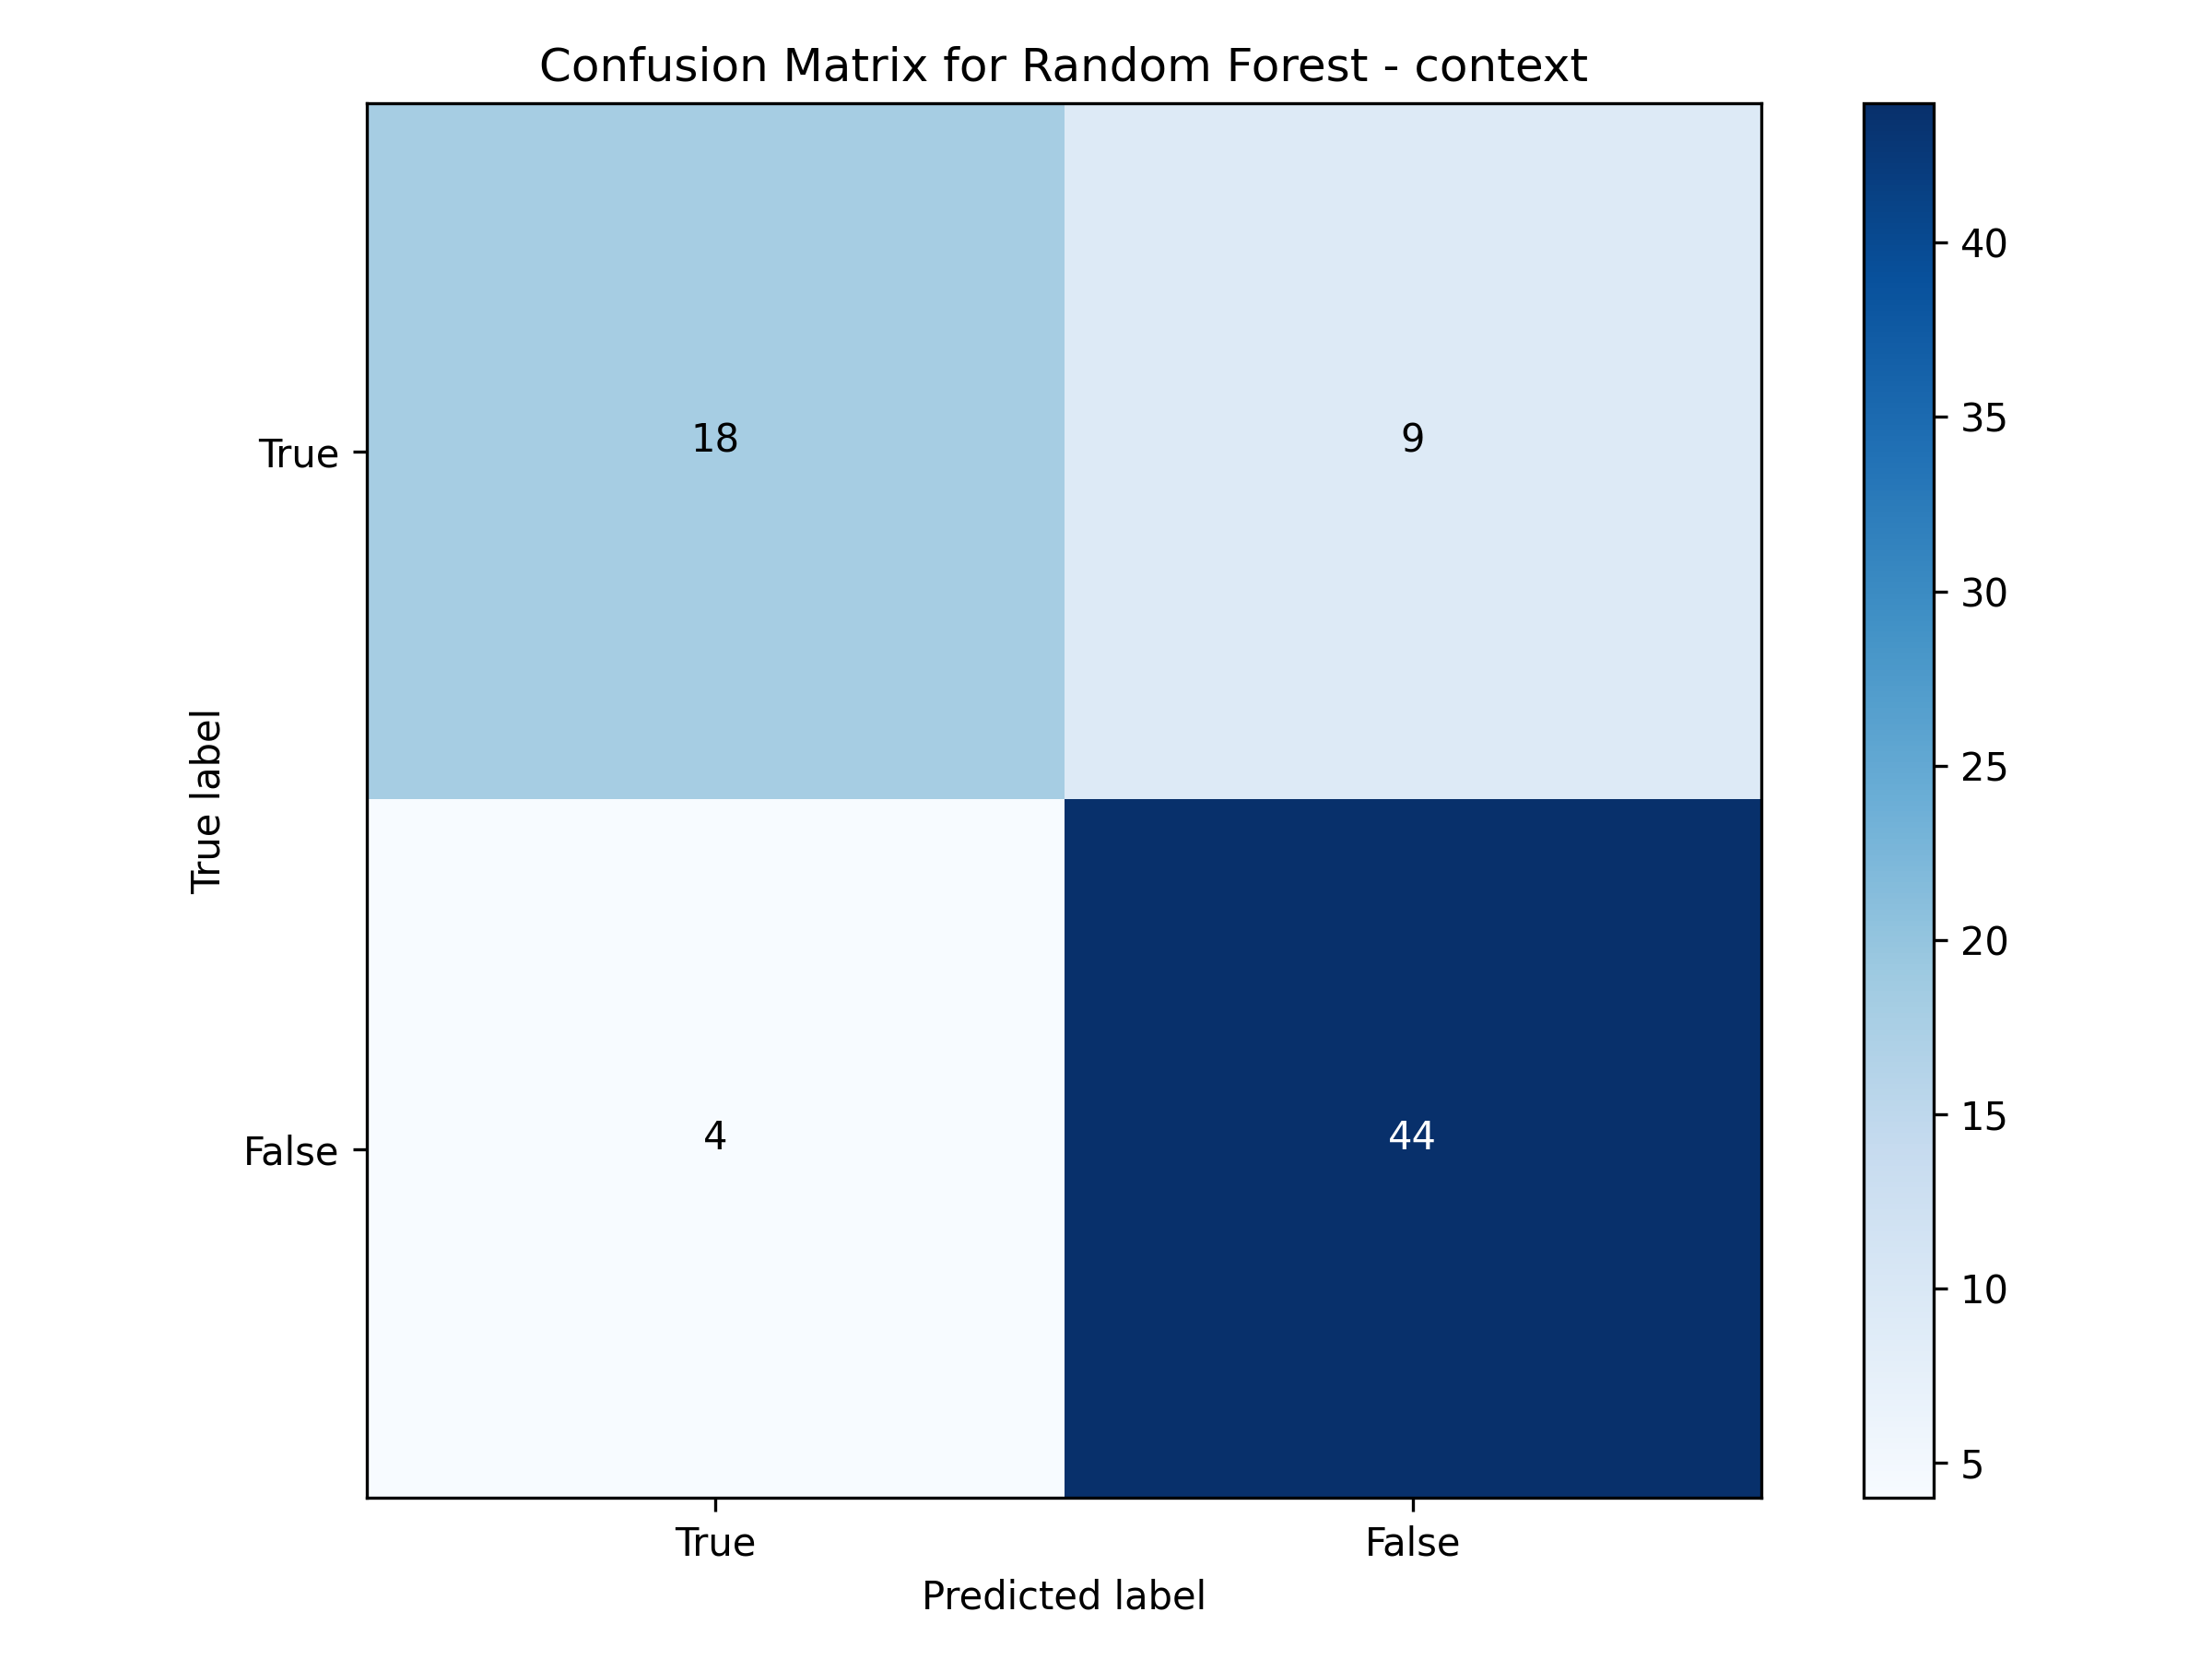
\includegraphics[width=\textwidth]{images/confusion_3.json-Random Forest_context_confusion_matrix}
        \label{fig:confusion_3_2}
    \end{minipage}
    \hspace{1em}
    \begin{minipage}[b]{0.45\textwidth}
        \centering
        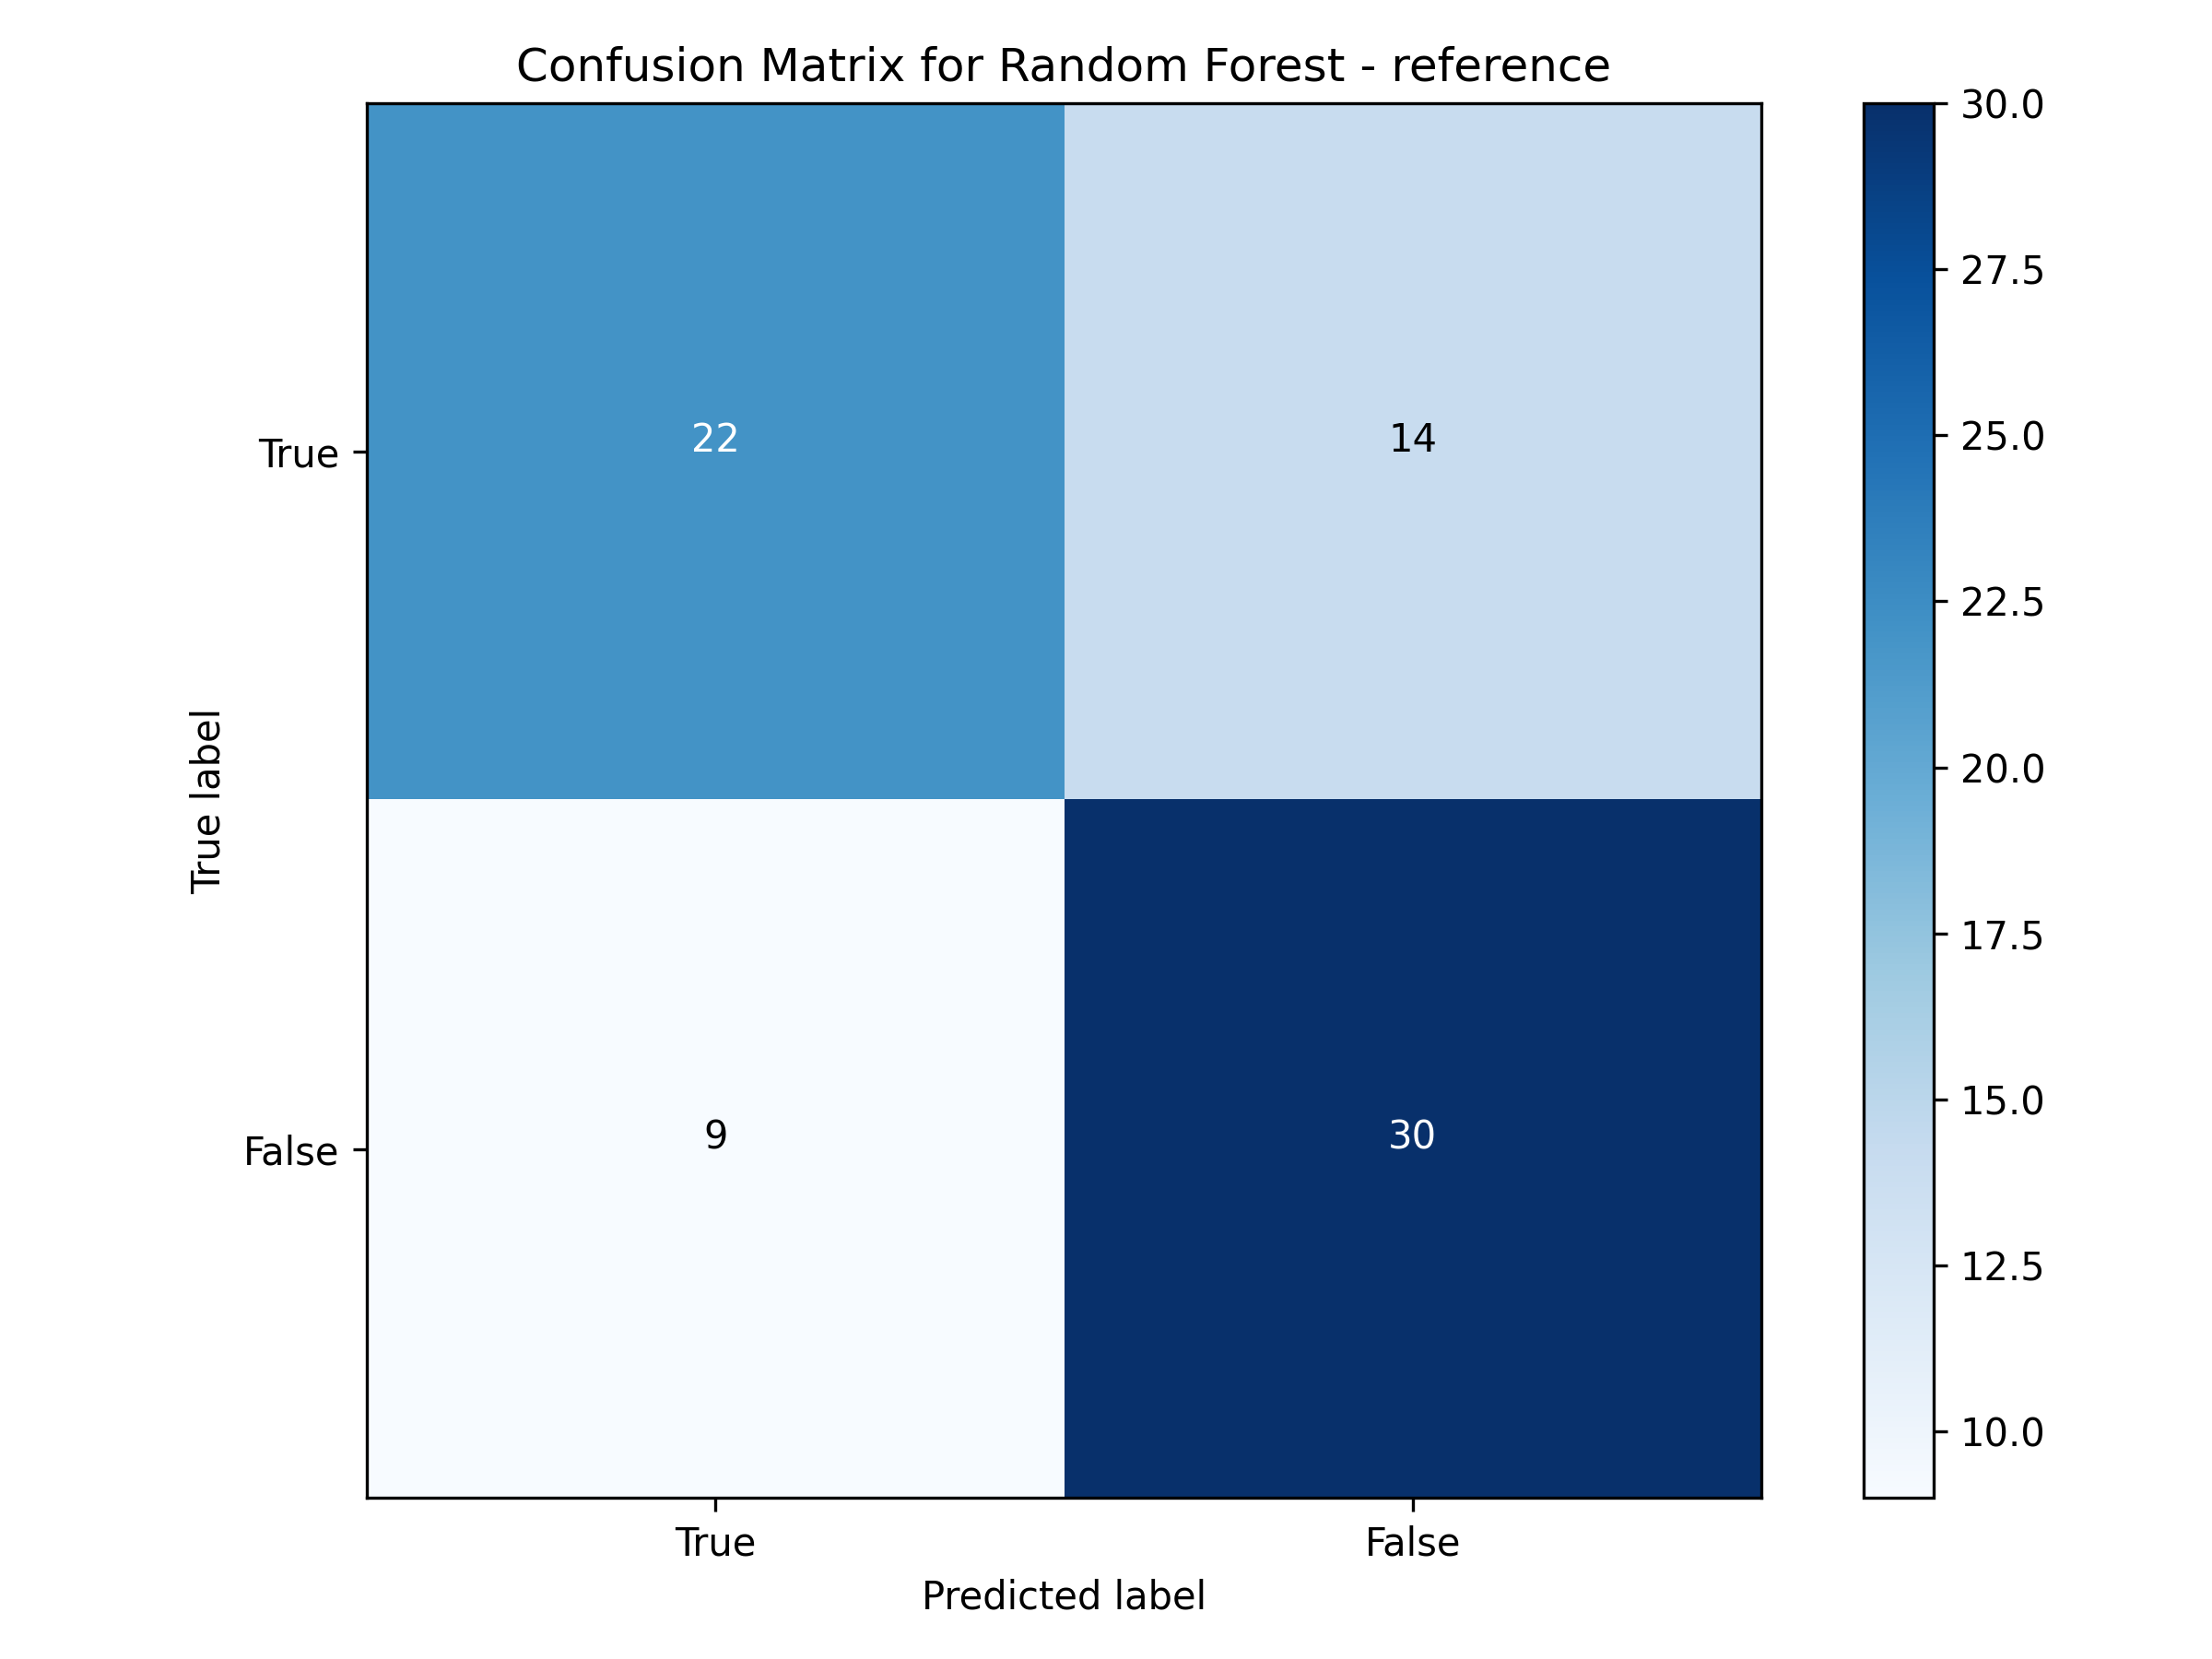
\includegraphics[width=\textwidth]{images/confusion_3.json-Random Forest_reference_confusion_matrix}
        \label{fig:confusion_3_3}
    \end{minipage}
    \caption{Matrice de confusion du modèle Random Forest pour la classification des tweets claim vs ref vs contexte.}
    \label{fig:confusion_3}
\end{figure}

    \newpage
    \section{Discussion}\label{sec:discussion}
    \subsection{Limites des Modèles}\label{subsec:limites-des-modeles}
Malgré des performances globalement satisfaisantes, chaque modèle présente certaines limites :
\begin{itemize}
  \item \textbf{Modèles linéaires (régression logistique, SVM) :} sensibles aux features bruitées ou non pertinentes, ils peuvent peiner à capturer des relations complexes dans les données textuelles.
  \item \textbf{Naive Bayes :} basé sur l’indépendance conditionnelle des features, il tend à sursimplifier les relations entre les mots et peut produire des résultats biaisés dans le cas de dépendances lexicales fortes.
  \item \textbf{k-NN :} sensible à la dimensionnalité et aux données bruitées, ce modèle peut être affecté par des mots non informatifs ou rares présents dans les tweets.
  \item \textbf{Random Forest :} bien qu’efficace, il peut sur-apprendre certains patterns lorsque le déséquilibre des classes n’est pas bien traité.
\end{itemize}

\subsection{Analyse des Features Importantes}\label{subsec:analyse-des-features-importantes}
Afin de mieux comprendre le comportement des modèles, nous avons extrait les features les plus importantes à l’aide du classifieur Random Forest.
Cette démarche nous a permis d’identifier les mots les plus discriminants entre les tweets scientifiques et non-scientifiques.
Ces termes ont ensuite été analysés en fonction de leur fréquence d’apparition, représentée sous forme de bar plot, ce qui a facilité l’interprétation des décisions du modèle et la compréhension des signaux textuels les plus informatifs.

\subsection{Inspection Manuelle des Erreurs}\label{subsec:inspection-manuelle-des-erreurs}
Pour les cas où les performances des modèles étaient jugées insuffisantes, une analyse manuelle des erreurs de classification a été réalisée.
Nous avons examiné les tweets mal classés, en particulier les faux positifs et faux négatifs, afin d’identifier des exemples ambigus ou potentiellement mal annotés.
Cette inspection a permis de mieux comprendre les limites des modèles face à des contenus complexes ou \textit{borderlines}.
Lorsque des motifs d’erreur récurrents ont été repérés, nous avons tenté d’ajuster le prétraitement des données ou d’équilibrer manuellement certaines combinaisons de labels.
Enfin, des modifications ciblées du pipeline ont été mises en place pour corriger ces erreurs, tout en veillant à ne pas nuire à la capacité de généralisation des modèles sur des données nouvelles.


    \newpage
    \section{Conclusion}\label{sec:conclusion}
    Cette étude a permis de comparer plusieurs modèles classiques de classification appliqués à des tweets selon leur rapport à la science.
Malgré les défis liés au bruit, à l’ambiguïté sémantique et au déséquilibre partiel des classes, les performances obtenues sont encourageantes.
Le modèle SVM s’est révélé le plus performant dans la majorité des tâches.
Mais plusieurs pistes d’amélioration peuvent être envisagées pour les travaux futurs.
Tout d’abord, l’intégration de modèles de langage pré-entraînés comme BERT ou CamemBERT pourrait permettre une meilleure prise en compte du contexte sémantique et améliorer la performance, notamment sur les classes minoritaires ou ambigües.
De plus, l’exploration de techniques de data augmentation textuelle ou de rééquilibrage plus avancé pour le multi-label (comme les algorithmes de suréchantillonnage spécifiques au texte) pourrait renforcer la robustesse des modèles face au déséquilibre des combinaisons de labels.
Enfin, une analyse plus fine des erreurs de classification, couplée à une révision éventuelle des annotations, permettrait d’améliorer la qualité du jeu de données, ce qui constitue une condition essentielle pour des modèles plus précis et interprétables.



    \newpage
    \section{Références}\label{sec:references}
    \printbibliography[heading=none]

    \newpage
    \section{Annexes}\label{sec:annexes}
    \input{sections/annexes}

\end{document}

